\documentclass[a4paper, 10pt]{article}
\usepackage[margin=1in]{geometry}
\usepackage{amsfonts, amsmath, amssymb, amsthm}
%\usepackage[none]{hyphenat}
\usepackage[utf8]{inputenc}
\usepackage[english, main=ukrainian]{babel}
\usepackage{pgfplots}
\usepgfplotslibrary{fillbetween}
\usepackage{bm}
\usepackage{physics}
\usepackage[unicode]{hyperref}
\usepackage{scalerel,stackengine}
\usepackage{multicol}
\usepackage{tikz-cd}
\usetikzlibrary{fit,matrix}
\usepackage{enumitem}
\usepackage{graphicx}

\usepackage{pdfpages}
\usepackage{caption}
\usepackage{float}
\usepackage{physics}
\usetikzlibrary{spy}
\usepackage{bbm}

\def\rightproof{$\boxed{\Rightarrow}$ }

\def\leftproof{$\boxed{\Leftarrow}$ }

\newtheoremstyle{theoremdd}% name of the style to be used
  {\topsep}% measure of space to leave above the theorem. E.g.: 3pt
  {\topsep}% measure of space to leave below the theorem. E.g.: 3pt
  {\normalfont}% name of font to use in the body of the theorem
  {0pt}% measure of space to indent
  {\bfseries}% name of head font
  {}% punctuation between head and body
  { }% space after theorem head; " " = normal interword space
  {\thmname{#1}\thmnumber{ #2}\textnormal{\thmnote{ \textbf{#3}\\}}}

\theoremstyle{theoremdd}
\newtheorem{theorem}{Theorem}[subsection]
\newtheorem{definition}[theorem]{Definition}
\newtheorem{example}[theorem]{Example}
\newtheorem{proposition}[theorem]{Proposition}
\newtheorem{remark}[theorem]{Remark}
\newtheorem{lemma}[theorem]{Lemma}
\newtheorem{corollary}[theorem]{Corollary}

\newcommand\thref[1]{\textbf{Th.~\ref{#1}}}
\newcommand\defref[1]{\textbf{Def.~\ref{#1}}}
\newcommand\exref[1]{\textbf{Ex.~\ref{#1}}}
\newcommand\prpref[1]{\textbf{Prp.~\ref{#1}}}
\newcommand\rmref[1]{\textbf{Rm.~\ref{#1}}}
\newcommand\lmref[1]{\textbf{Lm.~\ref{#1}}}
\newcommand\crlref[1]{\textbf{Crl.~\ref{#1}}}

\renewcommand{\qedsymbol}{$\blacksquare$}
\DeclareMathOperator{\linspan}{span}
\DeclareMathOperator{\Mat}{Mat}
\DeclareMathOperator{\ort}{ort}
\DeclareMathOperator{\pr}{pr}
\DeclareMathOperator{\evaluation}{ev}

\makeatletter
\renewenvironment{proof}[1][Proof.\\]{\par
\pushQED{\hfill \qed}%
\normalfont \topsep6\p@\@plus6\p@\relax
\trivlist
\item\relax
{\bfseries
#1\@addpunct{.}}\hspace\labelsep\ignorespaces
}{%
\popQED\endtrivlist\@endpefalse
}
\makeatother

\newcommand{\BigFig}[1]{\parbox{12pt}{\Huge #1}}
\DeclareMathOperator{\Bin}{Bin}
\DeclareMathOperator{\Geom}{Geom}
\DeclareMathOperator{\Pois}{Pois}
\DeclareMathOperator{\Exp}{Exp}
\DeclareMathOperator{\cov}{cov}
    	
\begin{document}
%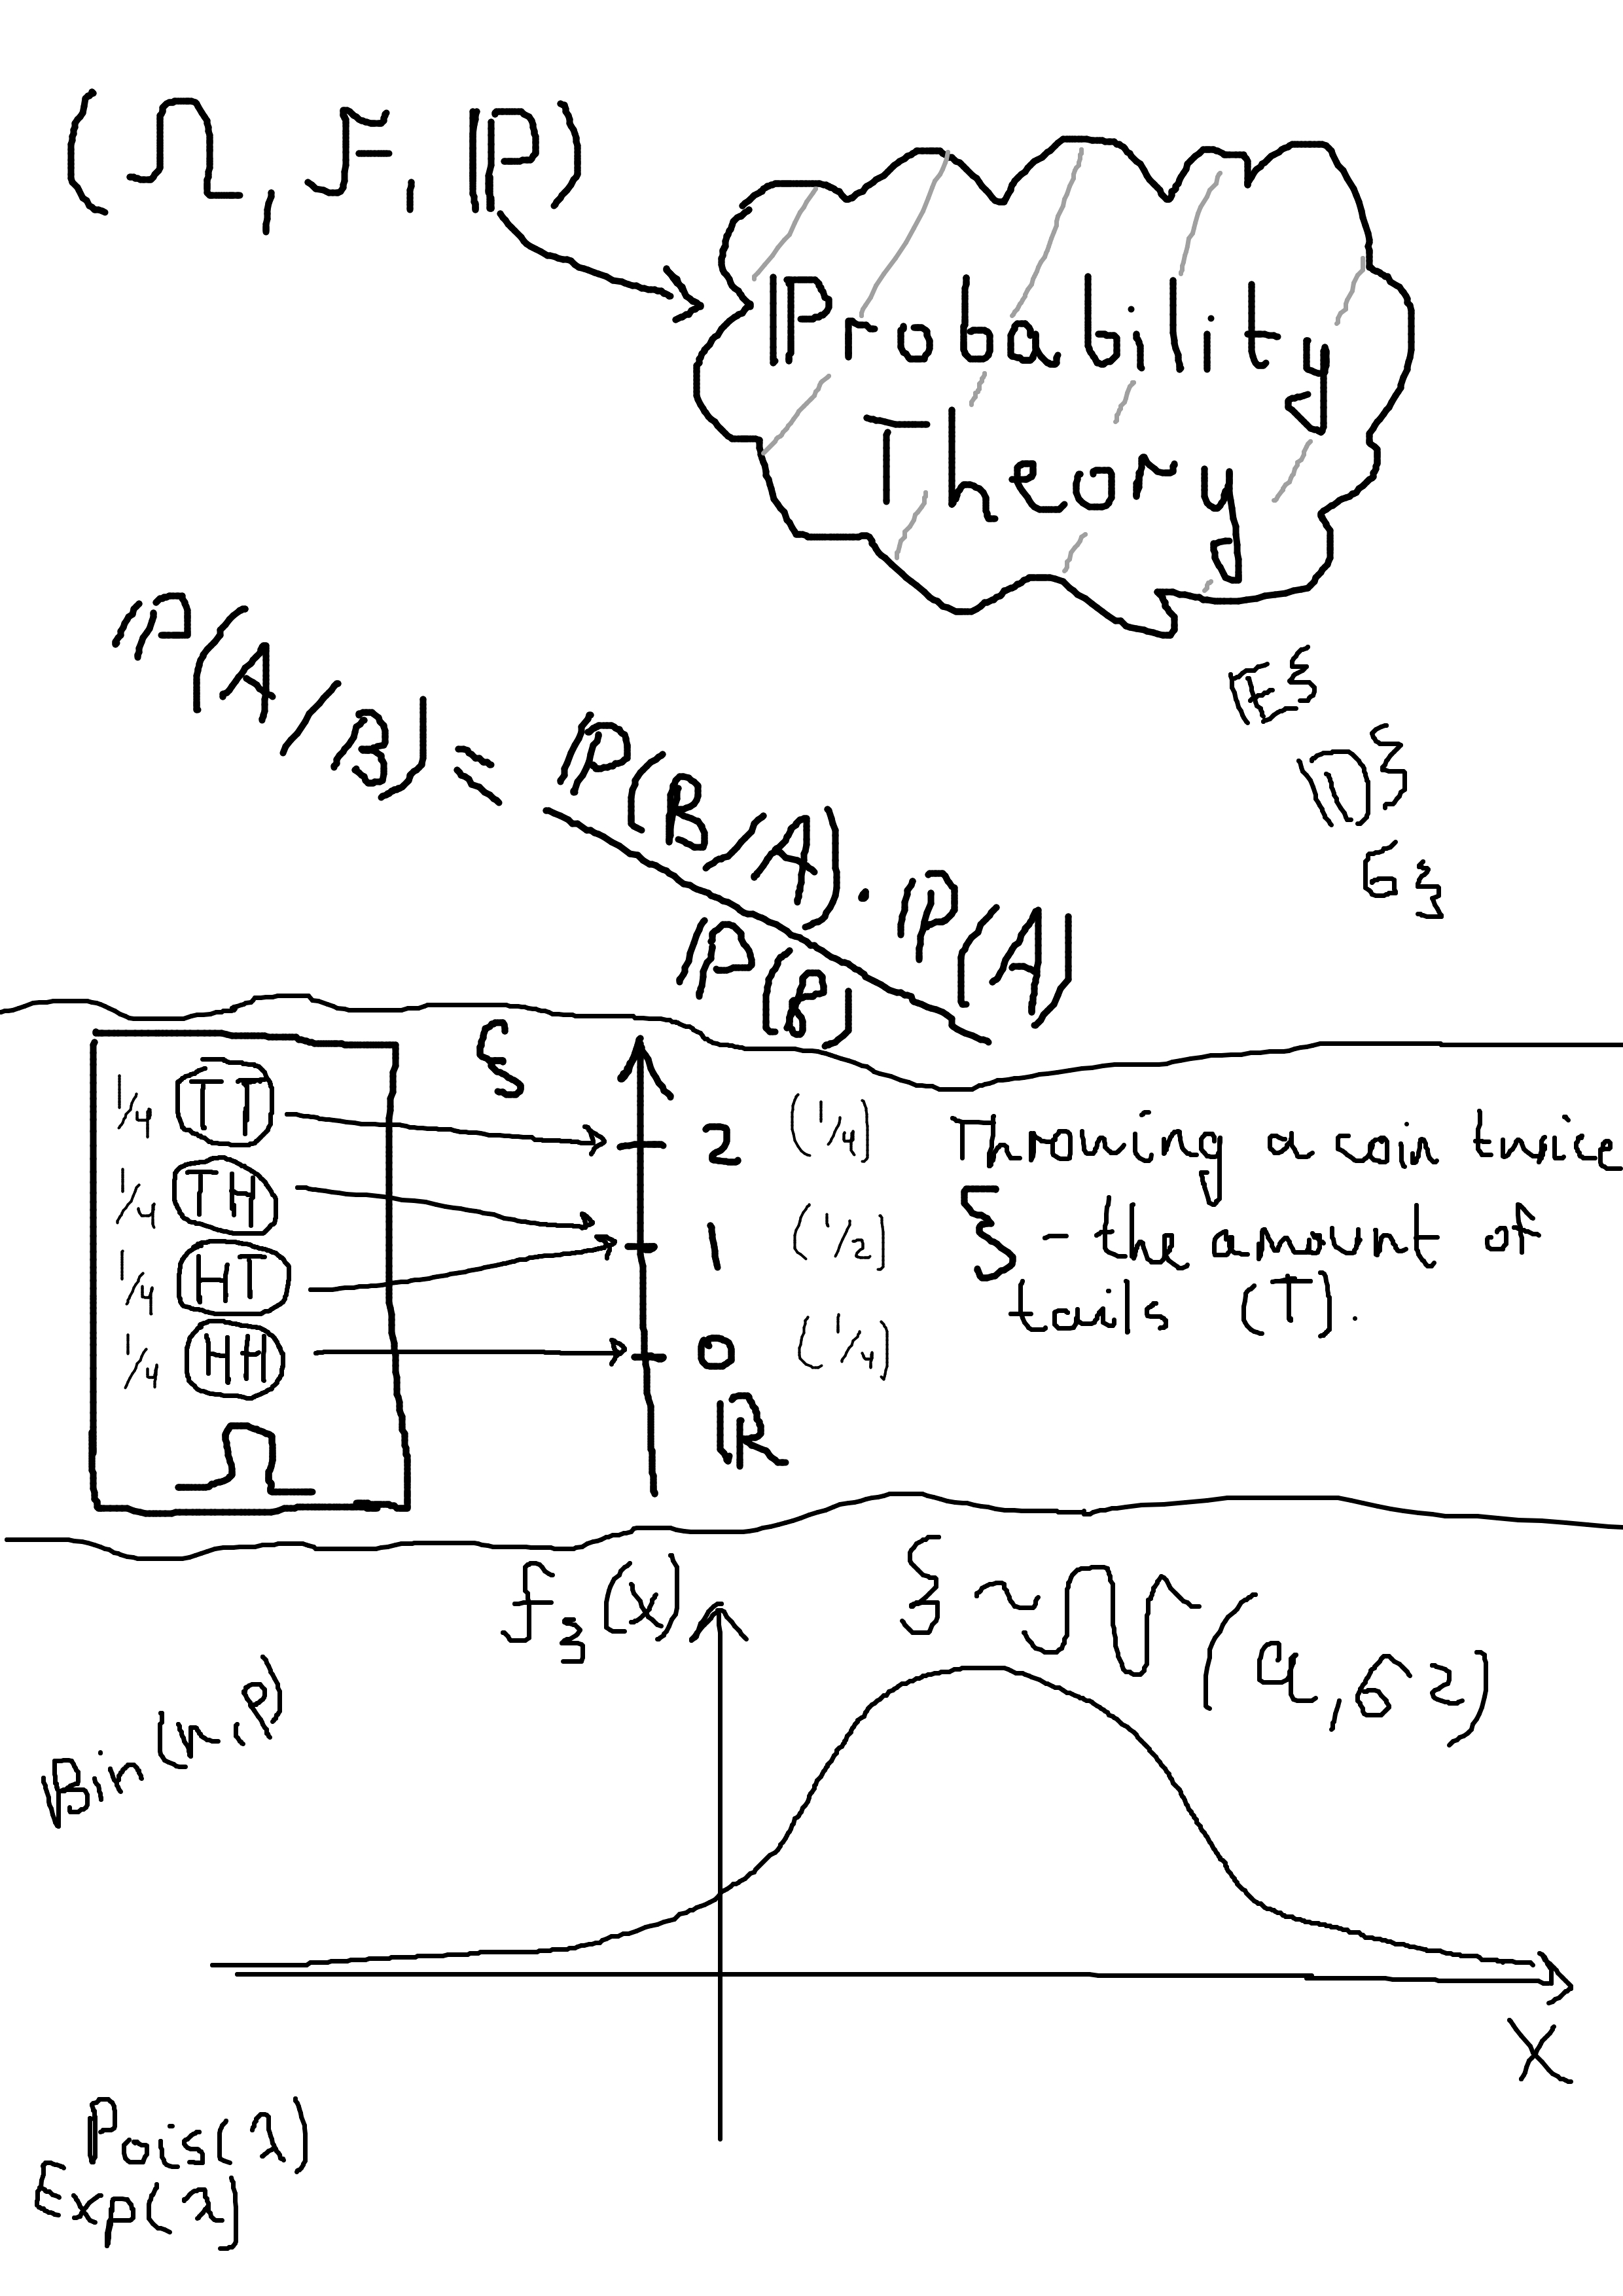
\includepdf[scale=1]{preview.jpg}
\tableofcontents
\newpage
    	
\section{Основи теорії ймовірності}
\subsection{Імовірнісний простір}
\begin{definition}
\textbf{Простором вибірок} (або часто називають \textbf{простором елементарних подій}) називають множину $\Omega$, яка складається з елементів $\omega \in \Omega$, які називаються \textbf{елементарними подіями}.
\end{definition}

\begin{example}
Кидаємо один раз монету, простір вибірок $\Omega$ складається з двох точок: $\Omega = \{H, T\}$, де $H = \text{head}$ (орел) та $T = \text{tail}$ (решка). \\
Ми виключаємо патові сценарії, коли монета впала на грань чи моента зникнула тощо.
\end{example}

\begin{example}
Кидаємо три рази монету, простір вибірок $\Omega$ уже буде такою:\\
$\Omega = \{ HHH, HHT, HTH, THH, HTT, THT, TTH, TTT \}$.
\end{example}

\begin{example}
Серед $M$ куль обираємо $n$ разів, після кожного вибору цю кулю повертаємо назад.\\
$\Omega = \{\omega : \omega = (a_1,\dots,a_n) \mid a_i = 1,\dots,M\}$, у цьому випадку $a_i$ -- це який м'яч ми взяли на $i$-му кроці обирання. Зауважимо, що $|\Omega| = M^n$. Вибірка $(a_1,\dots,a_n)$ в круглих дужках означає, що вона впорядкована. Тобто в цьому випадку порядок важливий.\\
$\Omega = \{\omega : \omega = [a_1,\dots,a_n] \mid a_i = 1,\dots,M\}$, у цьому випадку $a_i$ -- це який м'яч ми взяли на $i$-му кроці обирання. Зауважимо, що $|\Omega| = \widetilde{C}_M^n$. Вибірка $[a_1,\dots,a_n]$ в квадратних дужках означає, що вона невпорядкована. Тобто в цьому випадку порядок неважливий.
\end{example}

\begin{example}
Серед $M$ куль обираємо $n \leq M$ разів, після вибору цю кулю НЕ повертаємо назад.\\
$\Omega = \{\omega : \omega = (a_1,\dots,a_n) \mid a_k \neq a_l, k \neq l; a_i = 1,\dots,M\}$. Зауважимо, що $|\Omega| = A_M^n$.\\
$\Omega = \{\omega : \omega = [a_1,\dots,a_n] \mid a_k \neq a_l, k \neq l; a_i = 1,\dots,M\}$. Зауважимо, що $|\Omega| = C_M^n$.
\end{example}

\begin{example}
Опишемо зустріч двох осіб, що узгодили між собою зустрітися протягом однієї години. Позначимо за $x$ -- час приїзду першої особи; $y$ -- час приїзду другої особи. Маємо такий простір елементарних подій: $\Omega = \{ (x,y) : 0 \leq x \leq 1, 0 \leq y \leq 1\}$.
\end{example}

\begin{definition}
Задано $\Omega$ -- простір елементарних подій.\\
Підмножиною $A \subset \Omega$ будемо називати \textbf{випадковою подією}. Множина $\emptyset \subset \Omega$ називається \textbf{неможливою подією} (\textbf{impossible event}). Множина $\Omega \subset \Omega$ називається \textbf{достовірною подією} (\textbf{certain event}).
\end{definition}

\begin{example}
Кидаємо три рази монету, у нас $\Omega = \{ HHH, HHT, HTH, THH, HTT, THT, TTH, TTT \}$. Опишемо подію $A$, де хоча б два орла (head) випали. Це буде $A = \{HHT, HTH, THH, HHH\}$.
\end{example}
\noindent
Ми знаємо, що над множинами можна проводити операції: $\cup,\ \cap,\ $ взяття доповнення тощо. Якщо переформулювати це в жаргон теорії ймовірностей, то ми отримаємо наступний опис:\\
$A \cup B$ -- подія, яка відбудеться, коли хоча б одна з подій ($A$ або $B$) відбудеться.\\
$A \cap B$ -- подія, яка відбудеться, коли одночасно ці дві події ($A$ та $B$) відбудуться.\\
$A^c$ -- подія, яка відбудеться тоді, коли не відбудеться подія $A$.\\
$A \setminus B$ -- подія, яка відбудеться, коли спрацює подія $A$ та не спрацює подія $B$.

\begin{example}
Кидаємо двічі монету, маємо простір $\Omega = \{HH,HT,TH,TT\}$. Опишемо $A = \{HH,HT,TH\}$ -- випав хоча б один орел; $B = \{TT,TH,HT\}$ -- випала хоча б одна решка.\\
$A \cup B = \{HH,HT,TH,TT\} = \Omega$ -- випала або хоча б одна решка, або випав хоча б один герб (це зрозуміло, що буде достовірною подією).\\
$A \cap B = \{HT,TH\}$ -- випала хоча б одна решка та випав хоча б один герб.\\
$A^c = \{TT\}$ -- не випав жодний орел.
\end{example}

\begin{definition}
Події $A,B \subset \Omega$ називаються \textbf{несумісними}, якщо
\begin{align*}
A \cap B = \emptyset
\end{align*}
Події $A_1,A_2,\dots \subset \Omega$ називаються \textbf{попарно несумісними}, якщо
\begin{align*}
A_i \cap A_j = \emptyset,\ i \neq j
\end{align*}
\end{definition}

\begin{definition}
Маємо простір елементарних подій $\Omega$, створимо $\sigma$-алгебру $\mathcal{F}$ підмножин.\\
Така $\sigma$-алгебра називається \textbf{$\sigma$-алгеброю подій}. Вимірний простір $(\Omega,\mathcal{F})$ називають \textbf{вимірним простором стохастичного експерименту}.
\end{definition}

\begin{definition}
Задано $(\Omega,\mathcal{F})$ -- імовірнісний простір.\\
\textbf{Імовірністю} назвемо міру $\mathbb{P} \colon \mathcal{F} \to [0,+\infty)$, яка додатково має властивість:
\begin{align*}
\mathbb{P}(\Omega) = 1
\end{align*}
Трійка $(\Omega,\mathcal{F},\mathbb{P})$ називається \textbf{ймовірнісним простром}.
\end{definition}

\begin{proposition}[Властивості ймовірності]
Справедливе наступне:
\begin{enumerate}[nosep,wide=0pt,label={\arabic*)}]
\item $\mathbb{P}(A^c) = 1 - \mathbb{P}(A)$;
\item $\mathbb{P}(\emptyset) = 0$;
\item $A \subset B \implies \mathbb{P}(A) \leq \mathbb{P}(B)$;
\item $\mathbb{P}(A) \leq 1$;
\item $\mathbb{P}(B \setminus A) = \mathbb{P}(B) - \mathbb{P}(A)$;
\item $\mathbb{P}(A \cup B) = \mathbb{P}(A) + \mathbb{P}(B) - \mathbb{P}(A \cap B)$ (цю формулу можна узагальнити на довільне скінченне число множин, як це було з потужностями);
\item $\mathbb{P}$ неперервна зверху та знизу одночасно.
\end{enumerate}
\textit{Всі ці властивості -- це випливає з теорії міри.}
\end{proposition}

\subsection{Класична модель імовірності}
Припустимо, що $\Omega$ -- зліченний простір елементарних подій. Маємо $\mathbb{P}$ -- ймовірність, що задана на $\sigma$-алгебрі $\mathcal{F}$. У силу зліченності маємо наступне:\\
$\mathbb{P}(\Omega) = \displaystyle \mathbb{P}\left( \bigcup_{n=1}^\infty \{\omega_i\} \right) = \sum_{n=1}^\infty \mathbb{P}(\{\omega_i\})$.\\
Кожному $\omega_i \in \Omega$ поставимо число $\mathbb{P}(\{\omega_i\}) = p_i \geq 0$.\\
Тоді кожна подія $A$ має ймовірність $\mathbb{P}(A) = \displaystyle\sum_{\omega_i \in A} p_i$.
\bigskip \\
Всі ці процедури можна аналогічно повторити, якщо $\Omega$ -- скінченний простір.\\
Якщо $|\Omega| = k$ -- скінченний, то прийнято вважати, що всі елементарні події $\omega_i$ рівноможливі, тобто всі $p_1 = p_2 = \dots = p_k \overset{\text{позн.}}{=} p$ рівні. Це означатиме, що $\displaystyle\sum_{n=1}^k p_i = p_1 + \dots + p_k = k p = 1$. Отже, кожна ймовірність $p = \dfrac{1}{k}$.\\
Тоді кожна подія $A$ має ймовірність $\mathbb{P}(A) = \displaystyle\sum_{\omega_i \in A} p_i = \dfrac{m}{k}$, де $m$ -- кількість елементарних подій в $A$.\\
Отже, в класичній моделі ймовірності при $\Omega$ -- скінченна, ймовірність події обчислюється так:
\begin{align*}
\mathbb{P}(A) = \dfrac{|A|}{|\Omega|}
\end{align*}

\begin{example}
Кидаємо один раз монету, $\Omega = \{H,T\}$. Тоді в класичному сенсі $\mathbb{P}(\{H\}) = \mathbb{P}(\{T\}) \dfrac{1}{2}$. Тобто ймовірність випадіння орла чи решки -- рівноможлива.
\end{example}

\begin{example}
Кидаємо двічі монету. Знайти ймовірність того, що хоча б один орел випаде.\\
Маємо $\Omega = \{HH,HT,TH,TT\}$, описана подія $A = \{HH,HT,TH\}$. Тоді звідси $\mathbb{P}(A) = \dfrac{3}{4}$.
\end{example}

\begin{example}[Задача про буху секретарку]
Секретарка поклала $n$ листів в $n$ чистих конвертів, заклеїла ці конверти та посля цього написала адреси. Знайти ймовірність того, що хоча б один з листів дійде за призначенням.\\
Позначимо $A_i$ -- подія, де $i$-ий лист дійшов за призначенням. Тоді маємо, що $\mathbb{P}(A_j) = \dfrac{1}{n}$.\\
Маємо подію $A$ -- подія, де хоча б один з листів дійде за призначенням. Тобто $A = \displaystyle\bigcup_{i=1}^n A_i$.\\
$\mathbb{P}(A_i) = \dfrac{1}{n}$;\\
$\mathbb{P}(A_i \cap A_j) = \dfrac{1}{n(n-1)}$;\\
$\mathbb{P}(A_i \cap A_j \cap A_k) = \dfrac{1}{n(n-1)(n-2)}$;\\
$\vdots$\\
$\mathbb{P}(A_1 \cap \dots \cap A_n) = \dfrac{1}{n!}$.\\
Звідси випливає, що за формулою включення-виключення,\\
$\mathbb{P}(A) = n \cdot \dfrac{1}{n} - C_n^2 \dfrac{1}{n(n-1)} + \dots + (-1)^{n-1} \dfrac{1}{n!} = 1 - \dfrac{1}{2!} + \dfrac{1}{3!} - \dots + (-1)^{n-1} \dfrac{1}{n!}$.\\
Спрямуємо $n \to \infty$, зауважимо, що $e^{-1} = 1 - \dfrac{1}{1!} + \dfrac{1}{2!} - \dfrac{1}{3!} + \dots$ Тоді звідси $\displaystyle\lim_{n \to \infty} \mathbb{P}(A) = 1 - \dfrac{1}{e} \approx 0.63$.
\end{example}

\subsection{Умовна ймовірність}
\begin{definition}
Маємо $(\Omega, \mathcal{F}, \mathbb{P})$ -- ймовірнісний простір. Припустимо, що подія $B$ має ймовірність $\mathbb{P}(B) > 0$ -- деяка умова.\\
Імовірність події $A$ за умовою, що спрацювала подія $B$, називається \textbf{умовною ймовірністю $A$ за умовою $B$}. Обчислюється за такою формулою:
\begin{align*}
\mathbb{P}(A|B) = \dfrac{\mathbb{P}(A \cap B)}{P(B)}
\end{align*}
\end{definition}

\begin{example}
Кидаємо дві гральні кістки d6. Ми хочемо знайти ймовірність того, що випаде більше шести очок за умовою, що перша кістка повернула три очки.\\
Маємо простір $\Omega = \{ \omega: \omega = (a,b): 1 \leq a \leq 6, 1 \leq b \leq 6\}$.\\
$A$ -- подія, яка описує, що ми отримали більше шести очок (наприклад, $(4,6) \in A$);\\
$B$ -- подія, яка описує, що перша кістка дає три очки (наприклад, $(3,5) \in B$).\\
Тоді $\mathbb{P}(A|B) = \dfrac{\mathbb{P}(A \cap B)}{P(B)}$.\\
Зауважимо, що $\mathbb{P}(A \cap B) = \dfrac{|A \cap B|}{|\Omega|} = \dfrac{3}{36}$. У нас всього три події можливі: $(3,4),(3,5),(4,6)$.\\
Також маємо $\mathbb{P}(B) = \dfrac{|B|}{|\Omega|} = \dfrac{6}{36}$. Тут можливі шість подій: $(3,1), (3,2), \dots, (3,6)$.\\
Остаточно отримаємо ймовірність $\mathbb{P}(A|B) = \dfrac{3}{6} = \dfrac{1}{2}$.\\
Для порівняння, ймовірність того, що випаде більше шести очок (без жодних інших умов) $\mathbb{P}(A) = \dfrac{21}{36} = \dfrac{7}{12}$ -- вийшла більша ймовірність.
\end{example}

\begin{remark}
Зауважимо, що в класичному моделі $\mathbb{P}(A|B) = \dfrac{|A \cap B|}{|B|}$, якщо розписати кожну ймовірність.
\end{remark}

\begin{proposition}[Властивості умовної ймовірності]
Справедливе наступне:
\begin{enumerate}[nosep,wide=0pt,label={\arabic*)}]
\item $\mathbb{P}(A|A) = 1$;
\item $\mathbb{P}(\emptyset|A) = 0$;
\item $\mathbb{P}(A|B) = 1$, якщо $A \supset B$;
\item $\displaystyle \mathbb{P}\left(\bigsqcup_{n=1}^\infty A_n | B\right) = \sum_{n=1}^\infty \mathbb{P}(A_n | B)$.
\end{enumerate}
\textit{Вправа: довести.}
\end{proposition}

\begin{corollary}
Трійка $(\Omega \cap B, \mathcal{F} \cap B, \mathbb{P}(\cdot | B))$ задає ймовірнісний простір.
\end{corollary}

\subsection{Незалежність подій}
\begin{definition}
Події $A,B$ називаються \textbf{незалежними}, якщо
\begin{align*}
\mathbb{P}(A \cap B) = \mathbb{P}(A) \cdot \mathbb{P}(B)
\end{align*}
\end{definition}

\begin{proposition}[Властивості незалежних подій]
Нехай $A,B$ -- незалежні події. Справедливе наступне:
\begin{enumerate}[nosep,wide=0pt,label={\arabic*)}]
\item $\mathbb{P}(A|B) = \mathbb{P}(A)$ \qquad $\mathbb{P}(B|A) = \mathbb{P}(B)$;
\item $A,B^c$ або $A^c,B$ або $A^c,B^c$ -- також незалежні події;
\item Нехай $A,B$ та $A,C$ між собою незалежні та $B,C$ несумісні. Тоді $A, B \sqcup C$ -- незалежні.
\end{enumerate}
\textit{Вправа: довести.}
\end{proposition}

\begin{definition}
Події $A_1,\dots,A_n$ називаються \textbf{незалежними} (у сукупності), якщо
\begin{align*}
\forall i_1,\dots,i_r \in \{1,\dots,n\}: \mathbb{P}\left( \bigcap_{k=1}^r A_{i_k} \right) = \prod_{k=1}^r \mathbb{P}(A_{i_k})
\end{align*}
\end{definition}

\begin{definition}
Події $A_1,\dots,A_n$ називаються \textbf{попарно незалежними}, якщо
\begin{align*}
\forall i,j: i \neq j: \mathbb{P}(A_i \cap A_j) = \mathbb{P}(A_i) \cap \mathbb{P}(A_j)
\end{align*}
\end{definition}

\begin{remark}
Із того, що $A_1,\dots,A_n$ незалежні у сукупності, випливає, що $A_1,\dots,A_n$ -- попарно незалежні.\\
Проте навпаки не працює.
\end{remark}

\begin{example}[Приклад Бернштайна]
Маємо тетраедр, три грані якого розфарбовані відповідно червоним, зеленим та синім кольорами. Четверта грань -- комбінація цих трьох кольорів.\\
$R$ -- подія, коли тетраедр показує червоний колір після підкидання;\\
$G$ -- подія, коли тетраедр показує зелений колір після підкидання;\\
$B$ -- подія, коли тетраедр показує синій колір після підкидання.\\
Зауважимо спочатку, що $\mathbb{P}(R) = \mathbb{P}(G) = \mathbb{P}(B) = \dfrac{1}{2}$.\\
Події $R,G,B$ попарно незалежні. Дійсно, $\mathbb{P}(R \cap G) = \mathbb{P}(G \cap B) = \mathbb{P}(B \cap G) = \dfrac{1}{4}$.\\
Події $R,G,B$ не є незалежними у сукупності. Дійсно, $\mathbb{P}(R \cap G \cap B) = \dfrac{1}{4} \neq \dfrac{1}{8}$.
\end{example}

\subsection{Формула повної ймовірності}
Маємо $\Omega$ -- простір елементарних подій. Припустимо, що $H_1,H_2,\dots,H_n$ утворюють повну групу подій, у такому разі такі події називають \textbf{припущеннями}.\\
Нехай подія $A$ відбувається разом з якимось припущенням. Тоді\\
$\displaystyle \mathbb{P}(A) = \mathbb{P}\left(A \cap \Omega\right) = \mathbb{P}( A \cap (H_1 \sqcup \dots \sqcup H_n) = \mathbb{P}((A \cap H_1) \sqcup \dots \sqcup (A \cap H_n)) = \sum_{k=1}^n \mathbb{P}(A \cap H_k) = \sum_{k=1}^n \mathbb{P}(H_k) \mathbb{P}(A|H_k)$.\\
Таким чином, ми отримали формулу повної ймовірності:
\begin{align*}
\mathbb{P}(A) = \sum_{k=1}^n \mathbb{P}(H_k) \mathbb{P}(A|H_k)
\end{align*}

\begin{example}
У магазин постачають $80\%$ телефонів з Китаю, $15\%$ з В'єтнаму, $5\%$ з Південної Кореї. Із кожної країни кількість бракованих відповідно $1\% ,\ 0.1\% ,\ 0.01\%$. Обчислити ймовірність того, що куплений телефон буде бракованим.\\
$H_1$ -- подія, де телефон із Китаю;\\
$H_2$ -- подія, де телефон із В'єтнаму;\\
$H_3$ -- подія, де телефон із Південної Кореї.\\
Позначимо $A$ -- подія, де куплений телефон бракований (тут не зазначається, із якої країни ми купляємо телефон). Оскільки $H_1,H_2,H_3$ утворюють повну групу подій, то звідси\\
$\mathbb{P}(A) = \mathbb{P}(H_1) \mathbb{P}(A|H_1) + \mathbb{P}(H_2) \mathbb{P}(A|H_2) + \mathbb{P}(H_3) \mathbb{P}(A|H_3)$.\\
Зауважимо, що $\mathbb{P}(H_1) = 0.8,\ \mathbb{P}(H_2) = 0.15,\ \mathbb{P}(H_3) = 0.05$ (за умовою).\\
Також зазначимо, що $\mathbb{P}(A|H_1) = 0.01,\ \mathbb{P}(A|H_2) = 0.001,\ \mathbb{P}(A|H_3) = 0.0001$.\\
Отже, підставивши всі значення, отримамо $\mathbb{P}(A) = 0.008155$.
\end{example}

\subsection{Формула Баєса}
Маємо $\Omega$ -- простір елементарних подій. Припустимо, що $H_1,H_2,\dots,H_n$ утворюють повну групу подій, у такому разі такі події називають \textbf{припущеннями}.\\
У результаті проведення експерименту відбулася подія $A$. Виникає питання: чому дорівнює $\mathbb{P}(H_1|A),\dots,\mathbb{P}(H_n|A)$?\\
$\mathbb{P}(H_i|A) = \dfrac{\mathbb{P}(H_i \cap A)}{\mathbb{P}(A)} = \dfrac{\mathbb{P}(H_1) \mathbb{P}(A|H_i)}{\sum_{k=1}^n \mathbb{P}(H_k) \mathbb{P}(A|H_k)}$.\\
Таким чином, отримали формулу Баєса:
\begin{align*}
\mathbb{P}(H_i|A) = \dfrac{\mathbb{P}(H_1) \mathbb{P}(A|H_i)}{\displaystyle\sum_{k=1}^n \mathbb{P}(H_k)\mathbb{P}(A|H_k)}
\end{align*}
Така формула дає відповідь на питання, чому дорівнює ймовірність того, що мала місце кожна з гіпотез $H_i$, якщо вже подія $A$ сталася.

\subsection{Поліноміальна схема}
Нехай $A_1,\dots,A_k$ утворюють повну групу подій, позначимо їхні ймовірності $\mathbb{P}(A_i) = p_i$.\\
Проводимо експеримент $n$ разів, в кожному з яких відбувається одна з подій $A_i$. Задача: знайти ймовірність того, що:\\
подія $A_1$ виникне $m_1$ разів;\\
подія $A_2$ виникне $m_2$ разів;\\
$\vdots$\\
подія $A_k$ виникне $m_k$ разів.\\
Зрозуміло, що тут $m_1 + m_2 + \dots + m_k = n$. Також допускається, що одна з подій може не відбутися.\\
Таку ймовірність позначу за $\mathbb{P}_n(m_1,m_2,\dots,m_k)$.\\
Якщо згадати комбінаторику, то ми отримаємо таку формулу:
\begin{align*}
\mathbb{P}_n(m_1,\dots,m_k) = \dfrac{n!}{m_1! m_2! \dots m_k!} p_1^{m_1} p_2^{m_2} \dots p_k^{m_k}
\end{align*}
Така ймовірність називається поліноміальною.
\newpage

\section{Випадкові величини}
\subsection{Перші означення}
\begin{definition}
Заданий $(\Omega,\mathcal{F})$ -- вимірний простір, також розглянемо $(\mathbb{R}, \mathcal{B}(\mathbb{R}))$.\\
Функція $\xi \colon \Omega \to \mathbb{R}$ називається \textbf{випадковою величиною}, якщо
\begin{align*}
\xi \text{ -- $\mathcal{F}$-вимірна функція.}
\end{align*}
\end{definition}
\noindent
Оскільки $\xi$ -- $\mathcal{F}$-вимірна функція, то це (із курсу теорії міри) дозволяє сказати нам, що $\{\xi < a\} \in \mathcal{F},\ \{\xi \leq a \} \in \mathcal{F},\ \{\xi \geq a\} \in \mathcal{F},\ \{\xi > a \} \in \mathcal{F}$ для будь-якого $a \in \mathbb{R}$. Таке означення зумовлено тим, щоб ми мали змогу обчислювати (наприклад) $\mathbb{P}(\xi \in [a,b])$.

\begin{example}
Розглянемо модель підкидання монети двічі. Визначимо випадкову величину $\xi$ -- кількість решок (tail). Нагадаю, що $\Omega = \{HH,HT,TH,TT\}$. У такому разі випадкова величина діє таким чином:\\
$\xi(HH) = 0$ \qquad $\xi(HT) = \xi(TH) = 1$ \qquad $\xi(TT) = 2$.
\begin{figure}[H]
\centering
\begin{tikzpicture}
\draw (0,0) rectangle (2.5,4.5);
\foreach \i in {1,2,3,4}
	\draw[blue] (1.25,\i) circle (0.35);
\node[blue] at (1.25,1) {$HH$};
\node[blue] at (1.25,2) {$HT$};
\node[blue] at (1.25,3) {$TH$};
\node[blue] at (1.25,4) {$TT$};
\foreach \i\j in {1,2,3,4}
	\node at (0.5, \i) {$\frac{1}{4}$};
\node at (1.25,0.25) {$\Omega$};

\node at (4,0.25) {$\xi$};

\draw[->] (6,0)--(6,4.5) node at (6.25,0.25) {$\mathbb{R}$};
\foreach \i/\j [count=\x from 0] in {1/4,2/2,3/4}
	\draw ({6cm-2pt},\i*1.25)--({6cm+2pt},\i*1.25) node[anchor = west] {$\x ,\ (\frac{1}{\j})$};
	\draw[->] (1.6,1)--(6,{1*1.25});
	\draw[->] (1.6,2)--(6,{2*1.25});
	\draw[->] (1.6,3)--(6,{2*1.25});
	\draw[->] (1.6,4)--(6,{3*1.25});
\end{tikzpicture}
\caption*{Схематичне представлення функції розподілу. Кожній елементарній події ставиться ймовірність. Кожному числу кількості решок за два підкидання також ставиться своя ймовірність.}
\end{figure}
\end{example}

\begin{definition}
\textbf{Імовірнісним розподілом} випадкової величини $\xi$ називають таку міру:
\begin{align*}
P_\xi(B) = \mathbb{P}(\xi^{-1}(B)),\ B \in \mathcal{B}(\mathbb{R}),
\end{align*}
така міра визначена на просторі $(\mathbb{R}, \mathcal{B}(\mathbb{R}))$.
\end{definition}

\begin{definition}
\textbf{Функцією розподілу} випадкової величини $\xi$ називають таку функцію:
\begin{align*}
F_\xi(x) = \mathbb{P}\{\xi \leq x\},\ x \in \mathbb{R}
\end{align*}
\end{definition}

\begin{example}
Повернімося до підкидання монети двічі. Мали $\xi$ -- випадкова величина, що позначає кількість решок. Маючи всі дані вище, отримаємо таку функцію розподілу:\\
$F_{\xi}(x) = \begin{cases} 0, & x < 0 \\ \dfrac{1}{4}, & 0 \leq x < 1 \\ \dfrac{3}{4}, & 1 \leq x < 2 \\ 1, & x \geq 2 \end{cases}$.\\
Наприклад, чому при $x = 1.5$ ми маємо $F_\xi(1.5) = \dfrac{3}{4}$. Інтуїтивно кажучи, тут написана ймовірність того, що ми отримаємо не більше $1.5$ решок (тобто або одна решка, або жодну). Тобто $\mathbb{P}\{\xi \leq 1.5\} = \mathbb{P}\{\xi = 1\} + \mathbb{P}\{\xi = 0\} = \dfrac{1}{2} + \dfrac{1}{4} = \dfrac{3}{4}$.
\begin{figure}[H]
\centering
\begin{tikzpicture}
\draw[->] (-2,0)--(4,0) node[anchor = north] {$x$};
\draw[->] (0,-0.25)--(0,1.5) node[anchor = east] {$F_\xi(x)$};
\draw[->, red] (-2,0)--(0,0);
\draw[->, red] (0,{1/4})--(1,{1/4});
\draw[->, red] (1,{3/4})--(2,{3/4});
\draw[->, red] (2,1)--(4,1);
\draw (-1pt,1)--(1pt,1) node[scale = 0.6, anchor = east] {$1$};
\draw (-1pt,0.75)--(1pt,0.75) node[scale = 0.6, anchor = east] {$\frac{3}{4}$};
\draw (-1pt,0.25)--(1pt,0.25) node[scale = 0.6, anchor = east] {$\frac{1}{4}$};
\node[scale = 0.6] at (-0.1,-0.1) {$0$};
\draw (1,-1pt)--(1,1pt) node[scale = 0.6, anchor = north] {$1$};
\draw (2,-1pt)--(2,1pt) node[scale = 0.6, anchor = north] {$2$};
\end{tikzpicture}
\caption*{Графік функції розподілу випадкової величини.}
\end{figure}
\end{example}

\begin{proposition}[Властивості функції розподілу]
Справедливе наступне:
\begin{enumerate}[nosep,wide=0pt,label={\arabic*)}]
\item $F_\xi \in [0,1]$;
\item $F_\xi$ -- неспадна функція;
\item $\mathbb{P}\{\xi \in (x,y]\} = F_\xi(y) - F_\xi(x)$;
\item $F_\xi(x) \to 0$ при $x \to -\infty$; \qquad $F_\xi(x) \to 1$ при $x \to +\infty$;
\item $F_\xi \in C_{\text{right}}(\mathbb{R})$; 
\item $F_\xi(x-0) = \mathbb{P}\{\xi < x\}$.
\end{enumerate}
\end{proposition}

\begin{proof}
Доведемо кожну властивість окремо:
\begin{enumerate}[wide=0pt,label={\arabic*)}]
\item \textit{Випливає з того, які значення приймає ймовірність}.
\item Оберемо $x_1,x_2 \in \mathbb{R}$ такі, що $x_2 > x_1$. Тоді\\
$F_\xi(x_2) = \mathbb{P}\{\xi \leq x_2\} = \mathbb{P}\{ \{\xi \leq x_1\} \cup \{x_1 < \xi \leq x_2 \}\} = \mathbb{P}\{\xi \leq x_1\} + \mathbb{P}\{x_1 < \xi \leq x_2\} \geq F_\xi(x_1)$.
\item $\mathbb{P}\{\xi \in (x,y]\} = \mathbb{P}\{\xi \leq y\} - \mathbb{P}\{\xi \leq x\} = F_\xi(y) - F_\xi(x)$.
\item Розглянемо послідовність $\{x_n, n \geq 1\}$ така, що $x_n \to -\infty$, причому монотонно спадна (*). Зауважимо, що виконується такий ланцюг:\\
$\{\xi \leq x_{1}\} \supset \{\xi \leq x_{2}\} \supset \dots$\\
Отже, за теоремою про неперервність ймовірності, отримаємо наступне:\\
$\displaystyle\lim_{n \to \infty} F_\xi (x_{n}) = \lim_{n \to \infty} \mathbb{P}\{\xi \leq x_{n}\} = \mathbb{P} \left\{ \bigcap_{n=1}^\infty \{\xi \leq x_{n}\} \right\} = \mathbb{P}\{\emptyset\} = 0$.\\
Випадок, коли $F_\xi(x) \to 1$ при $x \to +\infty$, цілком аналогічний.
\item Нам треба довести, що $\displaystyle\lim_{x \to x_0+0} F_\xi(x) = F_\xi(x_0)$.\\
Оберемо послідовність $\{x_n, n \geq 1\}$ так, щоб $x_n \to x_0$ праворуч, причому монотонно спадає (*). Тоді знову ланцюг:\\
$\{\xi \leq x_1\} \supset \{\xi \leq x_2\} \supset \dots$\\
Отже, за теоремою про неперервність йомвірності, отримаємо наступне:\\
$\displaystyle\lim_{n \to \infty} F_\xi(x_n) = \lim_{n \to \infty} \mathbb{P}\{\xi \leq x_n\} = \mathbb{P} \left\{ \bigcap_{n=1}^\infty \{\xi \leq x_n\} \right\} = \mathbb{P} \{\xi \leq x_0\} = F_\xi(x_0)$.
\item Оберемо послідовність $\{x_n, n \geq 1\}$ така, що $x_n \to x_n$ ліворуч, причому монотонно зростає (*). Зауважимо, що виконується такий ланцюг:\\
$\{\xi \leq x_1\} \subset \{\xi \leq x_2\} \subset \dots$\\
Отже, за теоремою про неперервність ймовірності, отримаємо наступне:\\
$\displaystyle\lim_{n \to \infty} F_\xi(x_n) = \lim_{n \to \infty} \mathbb{P}\left\{ \xi \leq x_n\right\} = \mathbb{P}\left\{ \bigcup_{n=1}^\infty \{\xi \leq x_n\} \right\} = \mathbb{P}\{\xi < x_0\}$.
\end{enumerate}
Всі властивості доведені.
\end{proof}

\begin{remark}
Мабуть, я окремо прокоментую (*), чому нам досить саме спадної послідовності.\\
Розглянемо довільну $\{x_n,n \geq 1\}$ таку, що $x_n \to -\infty$. Простіше від супротивного.\\
!Припустимо, що $F_\xi(x_n) \not\to 0$ при $n \to \infty$, тоді існує $\varepsilon^* > 0$ такий, що $\forall N: \exists n \geq N: F_\xi(x_n) \geq \varepsilon^*$. Тоді звідси можна відокремили підпослідовність $\{x_{n_k}, k \geq 1\}$ так, щоб $x_{n_k} \to -\infty$, причому можна спадну взяти (бо $x_n \to -\infty$). Для спадних послідовностей уже знаємо, що $F_\xi(x_{n_k}) \to 0$. Але тоді $\exists K: \forall k \geq K: F_\xi(x_{n_k}) < \varepsilon^*$ -- суперечність!\\
Буде все аналогічно
\end{remark}

\begin{remark}
Особиве зауваження. Деякі досі визначають функцію розподілу таким чином:
\begin{align*}
F_\xi(x) = \mathbb{P}\{\xi < x\},\ x \in \mathbb{R}
\end{align*}
Тобто тут нерівність тепер строга. Глобально нічого не зміниться, окрім деяких властивостей. Наприклад, в цьому випадку функція $F_\xi \in C_{\text{left}}(\mathbb{R})$, але вже не справа.
\end{remark}

\subsection{Основні види випадкових величин}
\subsubsection{Дискретна випадкова величина}
\begin{definition}
Випадкова величина $\xi$ називається \textbf{дискретною}, якщо
\begin{align*}
\xi \text{ набуває скінченну чи зліченну кількість значень.}
\end{align*}
\end{definition}
\noindent Для того, щоб задати дискретну випадкову величину, крім значень випадкової величини ще треба мати ймовірності, із якими ці значення приймаються.\\
$p_i = P\{\xi^{-1}\{x_i\}\} = \mathbb{P}(\xi = x_i), \qquad \displaystyle\sum_{i=1}^\infty p_i = 1$.
\bigskip \\
Часто всі дані зручно записувати в \textbf{ряд розподілу}, що виглядає таким чином:
\begin{figure}[H]
\centering
\begin{tabular}{c|c|c|c|c|c}
$\xi$ & $x_1$ & $x_2$ & $\dots$ & $x_n$ & $\dots$ \\
\hline
$\mathbb{P}$ & $p_1$ & $p_2$ & $\dots$ & $p_n$ & $\dots$
\end{tabular}
\end{figure}
\noindent
Подивимося, як виглядає функція розподілу в такому разі:\\
$F_\xi(x) = \begin{cases}
0, & x < x_1 \\
p_1, & x_1 \leq x < x_2 \\
p_1 + p_2, & x_2 \leq x < x_3 \\
\vdots \\
p_1 + p_2 + \dots = 1, & x \geq x_n
\end{cases}$.\\
Графік даної функції розподілу буде просто ступінчата функція.

\begin{example}
Зокрема в нас був експеримент підкидання монети два рази. Встановлювали випадкову величину $\xi$ -- кількість решок. Це -- приклад дискретної випадкової величини, оскільки приймає три значення. Кожна з яких має власну ймовірність. Наведу ряд розподілу:
\begin{figure}[H]
\centering
\begin{tabular}{c|c|c|c}
$\xi$ & $0$ & $1$ & $2$ \\
\hline
$\mathbb{P}$ & $\dfrac{1}{4}$ & $\dfrac{1}{2}$ & $\dfrac{1}{4}$
\end{tabular}
\end{figure}
\noindent
Якщо просумувати всі ймовірності, то отримаємо одиницю -- тобто це справді ряд розподілу. Як вже було раніше зазначено, ми отримаємо ступінчату функцію розподілу. Не лінь ще раз намалювати.
\begin{figure}[H]
\centering
\begin{tikzpicture}
\draw[->] (-2,0)--(4,0) node[anchor = north] {$x$};
\draw[->] (0,-0.25)--(0,1.5) node[anchor = east] {$F_\xi(x)$};
\draw[->, red] (-2,0)--(0,0);
\draw[->, red] (0,{1/4})--(1,{1/4});
\draw[->, red] (1,{3/4})--(2,{3/4});
\draw[->, red] (2,1)--(4,1);
\draw (-1pt,1)--(1pt,1) node[scale = 0.6, anchor = east] {$1$};
\draw (-1pt,0.75)--(1pt,0.75) node[scale = 0.6, anchor = east] {$\frac{3}{4}$};
\draw (-1pt,0.25)--(1pt,0.25) node[scale = 0.6, anchor = east] {$\frac{1}{4}$};
\node[scale = 0.6] at (-0.1,-0.1) {$0$};
\draw (1,-1pt)--(1,1pt) node[scale = 0.6, anchor = north] {$1$};
\draw (2,-1pt)--(2,1pt) node[scale = 0.6, anchor = north] {$2$};
\end{tikzpicture}
\end{figure}
\end{example}

\subsubsection{Абсолютно неперервна випадкова величина}
\begin{definition}
Випадкова величина $\xi$ називається \textbf{неперервною}, якщо
\begin{align*}
F_\xi \in C(\mathbb{R})
\end{align*}
\end{definition}

\begin{proposition}
$\xi$ -- неперервна випадкова величина $\iff \forall x \in \mathbb{R}: \mathbb{P}\{\xi = x\} = 0$.
\end{proposition}

\begin{proof}
\rightproof Дано: $\xi$ -- неперервна випадкова величина, тобто $F_\xi \in C(\mathbb{R})$. Тоді звідси \\
$\mathbb{P}\{\xi = x\} = \mathbb{P}\{\xi \leq x\} - \mathbb{P}\{\xi < x\} = F_\xi(x) - F_\xi(x-0) = 0$.
\bigskip \\
\leftproof Дано: $\forall x \in \mathbb{R}: \mathbb{P}\{\xi = x\} = 0$. Іншими словами, $\mathbb{P}\{\xi = x\} = \mathbb{P}\{\xi \leq x\} - \mathbb{P}\{\xi < x\} = 0$, або ще іншими словами, $F_\xi(x) - F_\xi(x-0) = 0$. У силу неперервності справа отримаємо, що $F_\xi(x+0) = F_\xi(x-0)$, а тому функція неперервна в точці $x$, зокрема $F_\xi \in C(\mathbb{R})$.
\end{proof}

\begin{example}
Розглянемо координатну площину. Через точку $(0,1)$ під випадковим кутом $\alpha \in [0,\pi)$ (подія, що проведемо з таким кутом) проводимо пряму. Необхідно знайти точку перетину з $OX$. Згодом описати функцію розподілу.
\begin{figure}[H]
\centering
\begin{tikzpicture}
\draw[->] (-2,0)--(2,0) node[anchor = north] {$x$};
\draw[->] (0,-2)--(0,2) node[anchor = south] {$y$};
\draw[red] (1,2)--(-2,-1);
\fill (-1,0) circle (1pt) node[anchor = north] {$\xi$};
\fill (0,1) circle (1pt) node[anchor = east] {$(0,1)$};
\draw[dashed] (0,1)--(0.5,1);
\draw (0.5,1) arc (0:45:0.5) node[anchor = west] {$\alpha$};
\end{tikzpicture}
\end{figure}
\noindent Позначимо $\xi$ -- випадкова величина, що описує точку перетину з $OX$. Зауважимо, що $\ctg \alpha = \dfrac{-\xi}{1}$, тобто звідси $\xi = -\ctg \alpha$. Тепер обчислимо функцію розподілу.\\
$F_\xi(x) = \mathbb{P}\{\xi \leq x\} = \mathbb{P}\{-\ctg \alpha \leq x\} = \mathbb{P}\{\ctg \alpha \geq x\} = \mathbb{P}\{\alpha \in [0,\arcctg(-x)]\} = \\ = \mathbb{P}\{\alpha \in [0,\pi-\arctg x]\} = \dfrac{\pi - \arcctg x}{\pi} = 1 - \dfrac{\arcctg x}{\pi}$.
\end{example}
\noindent
У нас зараз виникає певна проблема. Імовірність потрапляння в будь-яку точку нулева. Спробуємо тоді оцінити ймовірність потрапляння в маленький окіл даної точки.

\begin{definition}
\textbf{Щільністю розподілу} неперервної випадкової величини $\xi$ називають границю
\begin{align*}
f_\xi(x) = \lim_{\Delta x \to 0} \dfrac{\mathbb{P}\{x \leq \xi < x + \Delta x\}}{\Delta x},
\end{align*}
якщо така границя існує.\\
Із означення та властивостей функцій розподілу випливає, що $f_\xi(x) = F'_\xi(x)$.\\
\textit{Увага! Дане означення не є строгим. Правильніше було би зробити таким чином.}
\end{definition}

\begin{definition}
Випадкова величина $\xi$ називається \textbf{абсолютно неперервною}, якщо
\begin{align*}
\exists f_\xi \colon \mathbb{R} \to \mathbb{R}: F_\xi(x) = \int_{-\infty}^x f_\xi(t)\,dt,
\end{align*}
водночас функція $f_\xi$ називається \textbf{щільністю розподілу}.
\end{definition}

\begin{remark}
$\xi$ -- абсолютно неперервна $\implies \xi$ -- неперервна.\\
На жаль, зворотне твердження не є вірним. Саме тому перше означення про щільність розподілу було нестрогим. Просто тому що не для всіх неперервних випадкових величин можна підібрати щільність розподілу. Це не єдина причина, там воно буде видно нижче.
\begin{figure}[H]
\centering
\begin{tikzpicture}
\draw [red] plot [smooth cycle] coordinates {(0,0) (1,1) (4,1) (4,0) (2,-1)} node at (3,0.5) {$\text{НВВ}$};
\draw [blue] plot [smooth cycle] coordinates {(0.5,0.5) (1.8,0.7) (1.7, -0.5)} node[scale=0.8] at (1.2,0.2) {$\text{АНВВ}$};
\end{tikzpicture}
\end{figure}
\noindent
\textit{TODO: додати приклад}
\end{remark}

\begin{proposition}[Властивості щільності розподілу]
Справедливе наступне:
\begin{enumerate}[nosep,wide=0pt,label={\arabic*)}]
\item $f_\xi = F'_\xi$;
\item $f_{\xi} \geq 0$;
\item $\displaystyle\int_{-\infty}^{+\infty} f_\xi(x)\,dx = 1$ (умова нормування);
\item $\displaystyle\mathbb{P}\{\xi \in \left<a,b\right>\} = \int_a^b f_\xi(x)\,dx$.
\end{enumerate}
\end{proposition}

\begin{proof}
Доведемо кожну властивість:
\begin{enumerate}[wide=0pt,label={\arabic*)}]
\item \textit{випливає з означення абсолютно неперервної випадкової величини}.
\item Оскільки $F_\xi$ то звідси випливає $f_{\xi} = F'_{\xi} \geq 0$.
\item $\displaystyle\int_{-\infty}^{+\infty} f_\xi(x)\,dx = \lim_{t \to +\infty} \int_{-\infty}^t f_\xi(x)\,dx = \lim_{t \to +\infty} F_\xi(t) = 1$.
\item $\displaystyle \mathbb{P}\{\xi \in \left<a,b\right>\} = F_\xi(b) - F_\xi(a) = \int_{-\infty}^b f_\xi(x)\,dx - \int_{-\infty}^a f_\xi(x)\,dx = \int_a^b f_\xi(x)\,dx$.
\end{enumerate}
Всі властивості доведені.
\end{proof}

\begin{example}
Повернімось до прикладу вище. Ми вже знайшли, чому дорівнює функція розподілу $F_\xi(x) = 1 - \dfrac{\arcctg x}{\pi}$. Можемо обчислити щільність -- отримаємо $f_\xi(x) = \dfrac{1}{\pi} \dfrac{1}{1+x^2}$. Зараз намалюємо графік та з'ясуємо зміст щільності.
\begin{figure}[H]
\centering
\begin{tikzpicture}
\draw[->] (-3,0)--(3,0) node[anchor = north] {$x$};
\draw[->] (0,-0.5)--(0,1.5) node[anchor = east] {$f_\xi(x)$};
\draw[domain=-3:3, smooth, variable=\x, red] plot ({\x}, {3/pi*1/(1+\x*\x)});
\node at (-0.5,1) {$\frac{1}{\pi}$};
\end{tikzpicture}
\caption*{Графік каже наступне. Найчастіше за всього ми будемо потрапляти в окіл точки $0$. Це означатиме, з точки зору нашої задачі, що точка перетину з $OX$ (а це наша $\xi$) буде частіше за всього неподалік від точки $0$.}
\end{figure}
\end{example}

\begin{example}
Нехай випадкова величина $\xi$ задається щільністю $f_\xi(x) = \begin{cases} a(2 - |x|), & x \in [-2,2] \\ 0, & \text{інакше} \end{cases}$. Знайти функцію розподілу та ймовірність того, що випадкова величина знаходиться в інтервалі $(1,5)$ (перед цією задачею треба з'ясувати, чому дорівнює $a \in \mathbb{R}$).\\
За умовою нормування, $\displaystyle\int_{-\infty}^{+\infty} f_\xi(x)\,dx = 1$, тобто площа має бути одиничною. Якщо намалювати схематично, то там буде рівнобедрений трикутник, площа якої $1 = S = \dfrac{1}{2} \cdot 4 \cdot 2a$. Отже, $a = \dfrac{1}{4}$.
\begin{figure}[H]
\centering
\begin{tikzpicture}
\draw[->] (-3,0)--(3,0) node[anchor = north] {$x$};
\draw[->] (0,-0.5)--(0,2.5) node[anchor = east] {$f_\xi(x)$};
\draw (2,-2pt)--(2,2pt) node[anchor = north] {$2$};
\draw (-2,-2pt)--(-2,2pt) node[anchor = north] {$-2$};
\draw (-2pt,2)--(2pt,2) node[anchor = east] {$2a$};
\draw[red] (-3,0)--(-2,0)--(0,2)--(2,0)--(3,0);
\end{tikzpicture}
\end{figure}
\noindent
Знайдемо тепер функцію розподілу, яка рахуєтсья як $F_\xi(x) = \displaystyle\int_{-\infty}^t f_\xi(t)\,dt$.\\
Якщо $x \in (-\infty,-2]$, то звідси $F_\xi(x) = \displaystyle\int_{-\infty}^x 0\,dt = 0$.\\
Якщо $x \in (-2,0]$, то звідси $F_\xi(x) = \displaystyle\int_{-\infty}^{-2} f_\xi(t)\,dt + \int_{-2}^x \dfrac{1}{4}(2+t)\,dt = \dots = \dfrac{x^2}{8} + \dfrac{x}{2} + \dfrac{1}{2}$.\\
Якщо $x \in (0,2]$, то звідси $F_\xi(x) = \displaystyle\int_{-\infty}^0 f_\xi(t)\,dt + \int_0^x \dfrac{1}{4}(2-t)\,dt = \left( \dfrac{0^2}{8} + \dfrac{0}{2} + \dfrac{1}{2} \right) + \int_0^x \dfrac{1}{4}(2-t)\,dt = \dots = -\dfrac{x^2}{8} + \dfrac{x}{2} + \dfrac{1}{2}$.\\
Якщо $x \in (2,+\infty)$, то звідси $F_\xi(x) = \displaystyle\int_{-\infty}^2 f_\xi(t)\,dt + \int_2^x 0\,dt = \left( -\dfrac{2^2}{8} + \dfrac{2}{2} + \dfrac{1}{2} \right) = 1$.\\
Власне, отримали $F_\xi(x) = \begin{cases} 0, & x \in (-\infty,-2] \\ \dfrac{x^2}{8} + \dfrac{x}{2} + \dfrac{1}{2}, & x \in (-2,0] \\ -\dfrac{x^2}{8} + \dfrac{x}{2} + \dfrac{1}{2}, & x \in (0,2] \\ 1, & x \in (2,+\infty) \end{cases}$.\\
Знайдемо тепер ймовірність. Це можна зробити двома способами, але зроблю це через функцію розподілу, раз її було вже знайдено. Тобто $\mathbb{P}\{\xi \in (1,5)\} = F_\xi(5) - F_\xi(1) = 1 - \dfrac{7}{8} = \dfrac{1}{8}$.
\bigskip \\
Порада як перевірити, що функція розподілу коректно знайдена:\\
1) продиференціювати назад та отримати ту саму щільність;\\
2) перерірити на неперервність функцію.
\end{example}

\subsection{Числові характеристики випадкових величин}
\subsubsection{Математичне сподівання}
\begin{definition}
\textbf{Математичним сподіванням} (або ще кажуть \textbf{середнім значенням}) випадкової величини $\xi$ називають таку величину:
\begin{align*}
\mathbb{E}\xi = \displaystyle\sum_{k=1}^\infty x_i p_i \text{ -- для дискретної величини} \\
\mathbb{E}\xi = \int_{-\infty}^{+\infty} x f_\xi(x)\,dx \text{ -- для неперервної величини}
\end{align*}
Математичне сподівання існує, якщо відбувається абсолютна збіжність (ряда або інтеграла залежно від ситуації).
\end{definition}

\begin{example}
Щоб кинути два кубики d6, нам треба заплатити $100$ грн. Якщо сума очок складає $7$ або $11$, то ми виграємо $400$ грн. Знайти можливий прибуток за одну гру.\\
Позначимо $\xi$ -- випадкова величина, яка відповідає за суму очок. Запишемо ряд розподілу в даній ситуації.
\begin{figure}[H]
\centering
\begin{tabular}{c|c|c|c|c|c|c|c|c|c|c|c}
$\xi$ & $2$ & $3$ & $4$ & $5$ & $6$ & $7$ & $8$ & $9$ & $10$ & $11$ & $12$ \\
\hline
$\mathbb{P}$ & $\dfrac{1}{36}$ & $\dfrac{1}{18}$ & $\dfrac{1}{12}$ & $\dfrac{1}{9}$ & $\dfrac{5}{36}$ & $\dfrac{1}{6}$ & $\dfrac{5}{36}$ & $\dfrac{1}{9}$ & $\dfrac{1}{12}$ & $\dfrac{1}{18}$ & $\dfrac{1}{36}$
\end{tabular}
\end{figure}
\noindent Позначимо $\eta$ -- випадкова величина, яка відповідає за прибуток після гри. Ряд розподілу виглядає так:
\begin{figure}[H]
\centering
\begin{tabular}{c|c|c}
$\eta$ & $0$ & $400$ \\
\hline
$\mathbb{P}$ & $\dfrac{7}{9}$ & $\dfrac{2}{9}$ 
\end{tabular}
\end{figure}
\noindent Зауважимо, що $\mathbb{P}\{\eta = 400\} = \mathbb{P}\{\xi = 7\} + \mathbb{P}\{\xi = 11\}$. Порахуємо тепер математичне сподівання:\\
$\mathbb{E}\eta = 0 \cdot \dfrac{7}{9} + 400 \cdot \dfrac{2}{9} = 88 \dfrac{8}{9}$.\\
Тобто це означає, що в будь-якому випадку ми будемо йти в мінус. Платимо $100$ грн, а очікується майже $89$ грн.
\end{example}

\begin{example}
У нас вже був приклад вище, де знайдена була щільність розподілу $f_\xi(x) = \dfrac{1}{\pi} \dfrac{1}{1+x^2}$. Тут математичне сподівання не знайти, оскільки $\mathbb{E}\xi = \displaystyle\int_{-\infty}^{+\infty} x f_\xi(x)\,dx$ -- розбіжний інтеграл.
\end{example}

\begin{definition}
Випадкові величини $\xi_1,\xi_2$, що задані на одному ймовірнісному просторами, називаються \textbf{незалежними}, якщо
\begin{align*}
\forall x,y: \{\xi_1 \leq x\} \text{ та } \{\xi_2 \leq y \} \text{ -- незалежні події.}
\end{align*}
Внаслідок чого можемо отримати $\mathbb{P}\{\xi_1 \leq x, \xi_2 \leq y\} = F_{\xi_1}(x) F_{\xi_2}(y)$.
\end{definition}

\begin{proposition}[Властивості математичних сподівань]
Справедливе наступне:
\begin{enumerate}[nosep,wide=0pt,label={\arabic*)}]
\item $\mathbb{E}c = c$, під математичним сподіванням мається на увазі стала випадкова величина $\xi \equiv c$;
\item $\mathbb{E}(\lambda \xi) = \lambda \mathbb{E} \xi,\ \lambda \in \mathbb{R}$;
\item $\mathbb{E}(\xi + \eta) = \mathbb{E}\xi + \mathbb{E}\eta$;
\item $\mathbb{E}(\xi_1 \xi_2) = \mathbb{E} \xi_1 \mathbb{E} \xi_2$ за умовою, що $\xi_1,\xi_2$ -- незалежні.
\end{enumerate}
\end{proposition}

\begin{proof}
Будемо доводити лише в випадку дискретної випадкової величини.
\begin{enumerate}[wide=0pt,label={\arabic*)}]
\item Випадкова величина $\xi \equiv c$, що дискретна, означає, що $\mathbb{P}\{\xi = c\} = 1$. Внаслідок чого, за означенням математичного сподівання, $\mathbb{E} c = c \cdot 1 = c$.
\item $\mathbb{E}(\lambda \xi) = \displaystyle\sum_{k=1}^\infty \lambda   x_i p_i = \lambda\sum_{k=1}^\infty x_i p_i = \lambda \mathbb{E} \xi$.
\item $\displaystyle\mathbb{E}(\xi + \eta) = \sum_{i,j}(x_i+y_j) p_{ij}$, де під ймовірністю $p_{ij} = \mathbb{P}\{\xi + \eta = x_i + y_j\}$.\\
Звідси випливає, що $\mathbb{E}(\xi + \eta) = \displaystyle x_i \sum_i \sum_j p_{ij} + y_i \sum_i \sum_j p_{ij}$.\\
Окремо розглянемо $\displaystyle\sum_{j} p_{ij} = \sum_{j} \mathbb{P}\{\xi + \eta = x_i + y_j\} \overset{\text{стверджую}}{=} \mathbb{P}\{\xi = x_i\} = p_i$. По-перше, зауважимо, що події $\{\xi + \eta = x_i + y_j\}, \forall j$ -- несумісні уже (це ясно). По-друге, нехай $\xi(\omega) + \eta(\omega) = x_i + y_{j_0}$, тоді обов'язково з цього випливає $\xi(\omega) = x_i$. Бо якби $\xi(\omega) \neq x_i$, то було би $\eta(\omega) \neq y_j, \forall j$, що неможливо. Отже, $\displaystyle\bigsqcup_j \{\xi + \eta = x_i + y_j\} = \{\xi = x_i\}$, а далі $\sigma$-адитивність ймовірності.\\
Аналогічно доведемо $\displaystyle\sum_{i} p_{ij} = \sum_{i} \mathbb{P}\{\xi + \eta = x_i + y_j\} = \mathbb{P}\{\eta = y_j\} = p_j$.\\
$\mathbb{E}(\xi + \eta) = \displaystyle\sum_{i} x_i p_i + \sum_{j} y_j p_j = \mathbb{E} \xi + \mathbb{E} \eta$.
\item $\mathbb{E}(\xi_1 \xi_2) = \displaystyle \sum_{i,j} (x_i y_j) \mathbb{P}\{\xi_1 \xi_2 = x_i y_j\} = \sum_{i,j} (x_i y_j) \mathbb{P} \{ \{\xi_1 = x_i\} \cap \{ \xi_2 = y_j\} \} \overset{\text{незалежність}}{=} \\
= \sum_{i,j} x_i p_i y_j p_j = \left( \sum_i x_i p_i \right) \left( \sum_j y_j p_j \right) = \mathbb{E}\xi_1 \mathbb{E}\xi_2$.
\end{enumerate}
Для неперервних випадкових величин доведення 3),4) буде пізніше.
\end{proof}

\subsubsection{Дисперсія, середньоквадратичне відхилення}
Задана випадкова величина $\xi$. Суть дисперсії полягає в тому, щоб охарактеризувати степінь розкиду значень $\xi$ навколо середнього $\mathbb{E}\xi$.
\begin{definition}
\textbf{Дисперсією} випадкової величини $\xi$ називають таку величину:
\begin{align*}
\mathbb{D}\xi = \mathbb{E}(\xi - \mathbb{E}\xi)^2
\end{align*}
\end{definition}

\begin{remark}
Випадкова величина $\xi - \mathbb{E}\xi$ -- це розкидані значення навколо нуля. Якщо будемо брати просто $\mathbb{E}(\xi - \mathbb{E}\xi)$, то це буде завжди нуль (через властивості можна довести), тому що є додатні значення та від'ємні, та усереднене буде нулевим. Тому ми додали другий степінь, щоб можна було з обох сторін брати додатні числа.
\end{remark}
\noindent
Розпишемо дисперсію більш детально:\\
$\mathbb{D}\xi = \mathbb{E}(\xi^2) - 2 \xi \mathbb{E}\xi + (\mathbb{E}\xi)^2) = \mathbb{E} \xi^2 - \mathbb{E}(2 \xi \mathbb{E}\xi) + \mathbb{E}(\mathbb{E}\xi)^2 = \mathbb{E}\xi^2 - 2 (\mathbb{E}\xi)^2 + (\mathbb{E}\xi)^2$.\\
Отже, дисперсія випадкової величини $\xi$ можна обчислити за такою формулою:
\begin{align*}
\mathbb{D}\xi = \mathbb{E}(\xi^2) - (\mathbb{E}\xi)^2
\end{align*}

\begin{proposition}[Властивості дисперсії]
Справедливе наступне:
\begin{enumerate}[nosep,wide=0pt,label={\arabic*)}]
\item $\mathbb{D}\xi \geq 0$;
\item $\mathbb{D}\xi = 0 \iff \xi \equiv c$;
\item $\mathbb{D}(c \xi) = c^2 \mathbb{D}\xi$;
\item $\mathbb{D}(\xi_1 + \xi_2) = \mathbb{D}\xi_1 + \mathbb{D}\xi_2$ за умовою, що $\xi_1,\xi_2$ -- незалежні.
\end{enumerate}
\textit{1) випливає з означення математичного сподівання та решта 2),3),4),5) випливають з другої формули.}
\end{proposition}

\begin{definition}
\textbf{Середньоквадратичним відхиленням} випадкової величини $\xi$ називають наступне:
\begin{align*}
\sigma_\xi = \sqrt{\mathbb{D}\xi}
\end{align*}
Це ще часто називають \textbf{стандартним відхиленням}. Характеризує, по суті, наскільки від середнього значення ми можемо відхилитися ліворуч чи праворуч.
\end{definition}

\begin{example}
Позначимо $\xi$ -- випадкова величина, яка описує кількість забитих м'ячів командою МЮ за останні $33$ матчі АПЛ сезону 23/24. На основі відомих даних знайти математичне сподівання та дисперсію.\\
У мене вийшов ось такий ряд розподілу, поки скролив усі матчі:
\begin{figure}[H]
\centering
\begin{tabular}{c|c|c|c|c|c}
$\xi$ & $0$ & $1$ & $2$ & $3$ & $4$ \\
\hline
$\mathbb{P}$ & $\dfrac{7}{33}$ & $\dfrac{10}{33}$ & $\dfrac{9}{33}$ & $\dfrac{5}{33}$ & $\dfrac{2}{33}$
\end{tabular}
\end{figure}
\noindent
Обчислимо дисперсію випадкової величини. Для цього спочатку знайдемо математичне сподівання та ще додатковий параметр.\\
$\mathbb{E}\xi = 0 \cdot \dfrac{7}{33} + 1 \cdot \dfrac{10}{33} + 2 \cdot \dfrac{9}{33} + 3 \cdot \dfrac{5}{33} + 4 \cdot \dfrac{2}{33} = \dfrac{51}{33} = 1 \dfrac{18}{33}$ (ну коротше, десь півтори м'ячи в середньому).\\
$\mathbb{E}\xi^2 = 0^2 \cdot \dfrac{7}{33} + 1^2 \cdot \dfrac{10}{33} + 2^2 \cdot \dfrac{9}{33} + 3^2 \cdot \dfrac{5}{33} + 4^2 \cdot \dfrac{2}{33} = \dfrac{123}{33} = 3 \dfrac{24}{33}$.\\
Отже, звідси $\mathbb{D}\xi = \mathbb{E}\xi^2 - \left( \mathbb{E}\xi \right)^2 \approx 1.33$. Відхилення $\sigma_\xi = \sqrt{\mathbb{D}\xi} \approx 1.15$. Тобто очікується зазвичай десь від $0.38$ до $2.7$ голів.
\end{example}

\subsection{Коротко про генератриси в теорії ймовірностей}
Припустимо, що випадкова величина $\xi \in \{0,1,2,\dots,\}$, на кожному значенні ймовірність відповідно $p_0,p_1,p_2,\dots$. Ми вже знаємо, що генератриса (generating function) послідовності $\{a_n, n \geq 0\}$ визначається як $G(a_n;z) = \displaystyle\sum_{n=0}^\infty a_n z^n$. Тепер візьмемо послідовність ймовірностей $\{p_n, n \geq 0\}$ -- отримаємо генератрису $G(p_n;z) = \displaystyle\sum_{n=0}^\infty p_n z^n \overset{\text{насправді}}{=} \mathbb{E}(z^{\xi})$.\\
Отже, маємо таке означення:
\begin{definition}
\textbf{Генератрисою випадкової величини} $\xi \in \{0,1,2,\dots\}$ називають наступне:
\begin{align*}
G_\xi(z) = \mathbb{E}(z^\xi)
\end{align*}
Англійською це називають \textbf{probability generating function}.
\end{definition}

\begin{proposition}[Властивості генератриси випадкової величини]
Справедливе наступне:
\begin{enumerate}[nosep,wide=0pt,label={\arabic*)}]
\item $G_\xi(z)$ визначений при $|z| \leq 1$ (ряд при таких $z$ рівномірно збіжний);
\item $G_\xi(1) = 1$;
\item $G_\xi$ -- неспадна;
\item $G_\xi \geq 0$;
\item Розподіл випадкової величини $\xi$ повністю визначається генератрисою $G_\xi(t)$;
\item Нехай $\xi,\eta$ -- незалежні. Тоді $G_{\xi + \eta}(z) = G_\xi(z) \cdot G_\eta(z)$;
\end{enumerate}
\end{proposition}

\begin{proof}
Доведемо окремо:
\begin{enumerate}[wide=0pt,label={\arabic*)}]
\item $|z^k p_k| \leq p_k$ при наших обраних $z$, а тому якщо розглянути ряд $\displaystyle\sum_{k=0}^\infty p_k = 1$ (який збіжний), то за мажорантною ознакою Ваєрштраса, $G_\xi(z) = \displaystyle\sum_{k=0}^\infty z_k p^k$ буде рівномірно збіжний при $|z| \leq 1$.
\item $G_\xi(1) = \displaystyle\sum_{k=0}^\infty p_k = 1$.
\item \textit{Зрозуміло}.
\item \textit{Зрозуміло}.
\item Дана властивість означає, що за допомогою генератриси ми можемо повністю відновити ряд розподілу. Тобто кожному значенню випадкової величини можемо відновити ймовірність. Доведемо, що $p_k = \dfrac{G_\xi^{(k)}(0)}{k!}$. Для цього ми просто диференціюємо (скільки треба), маємо права в силу того, що це степеневий ряд. А далі просто підставляємо $z = 0$.
\item $G_{\xi + \eta}(z) = \mathbb{E}(z^{\xi + \eta}) = \mathbb{E}(z^{\xi}z^{\eta}) = \mathbb{E}(z^\xi) \mathbb{E}(z^\eta) = G_\xi(z) G_\eta(z)$.\\
Єдине треба переконатися, що коли $\xi,\eta$ незалежні, то звідси $z^\xi, z^\eta$ теж незалежні. Це вже поясню, коли буду вводити строго через теорію міри.
\end{enumerate}
Всі властивості (майже чесно) довели.
\end{proof}

\begin{remark}
Зауважимо, що $\mathbb{E} \xi = G'_\xi(1)$ та $\mathbb{E}\xi^2 = G_\xi'(1) + G_\xi''(1)$. Це дозволить простіше обчислювати дисперсію.
\end{remark}

\subsection{Популярні розподіли дискретних випадкових величин}
\subsubsection{Розподіл Бернуллі}
Розподіл Бернуллі можна описати таким рядом розподілу:
\begin{figure}[H]
\centering
\begin{tabular}{c|c|c}
$\xi$ & $0$ & $1$ \\
\hline
$\mathbb{P}$ & $q$ & $p$
\end{tabular}
\end{figure}
\noindent
У цьому випадку $p+q = 1$.\\
Тобто розподіл Бернуллі характеризує успіх виконання даної події чи невдачі.\\
Функція розподілу даної випадкової величини буде виглядати таким чином:\\
$F_\xi(x) = \begin{cases} 0, & x < 0 \\ q, & 0 \leq x < 1 \\ 1, & x \geq 1 \end{cases}$.\\
Якщо обчислити математичне сподівання та дисперсію, то отримаємо таку формулу:\\
$\mathbb{E}\xi = p, \qquad \mathbb{D}\xi = pq$.

\subsubsection{Біноміальний розподіл}
Біноміальний розподіл можна описати таким рядом розподілу:
\begin{figure}[H]
\centering
\begin{tabular}{c|c|c|c|c|c|c}
$\xi$ & $0$ & $1$ & $\dots$ & $k$ & $\dots$ & $n$ \\
\hline
$\mathbb{P}$ & $q^n$ & $n p q^{n-1}$ & $\dots$ & $C_n^k p^k q^{n-k}$ & $\dots$ & $p^n$
\end{tabular}
\end{figure}
\noindent
Біноміальний розподіл описує кількість успіхів у схемі Бернуллі з $n$ випробувань та з імовірністю успіху $p$. Такий ряд розподілу можна ось так коротко записати: $\xi \sim \Bin(n,p)$.\\
Мабуть, писати функцію розподілу такої випадкової величини не буду, бо тут ясно цілком, що буде. Краще обчислю детально математичне сподівання разом із дисперсією.\\
Оскільки $\xi \in \{0,1,2,\dots\}$, то ми можемо все це зробити через генератриси.\\
$G_\xi(z) = \displaystyle\sum_{k=0}^n p_k z^k = \displaystyle\sum_{k=0}^n C_n^k p^k q^{n-k} z^k = \sum_{k=0}^n C_n^k (pz)^k q^{n-k} = (pz+q)^n$.\\
Зокрема звідси $G'_\xi(z) = pn(pz+q)^{n-1}$, а також $G''_\xi(z) = p^2 n(n-1)(pz+q)^{n-2}$. Тепер можемо спокійно знайти бажані параметри.\\
$\mathbb{E}\xi = pn(p \cdot 1 + q) = pn$.\\
$\mathbb{D}\xi = pn + p^2n(n-1) - p^2n^2 = np + n^2p^2 - n^2p^2 -np^2 = np(1-p) = npq$.\\
Отже, отримали:\\
$\mathbb{E}\xi = np, \qquad \mathbb{D}\xi = npq$.

\subsubsection{Геометричний розподіл}
Геометричний розподіл можна описати таким рядом розподілу:
\begin{figure}[H]
\centering
\begin{tabular}{c|c|c|c|c|c}
$\xi$ & $0$ & $1$ & $\dots$ & $k$ & $\dots$ \\
\hline
$\mathbb{P}$ & $p$ & $qp$ & $\dots$ & $q^kp$ & $\dots$ \\
\end{tabular}
\end{figure}
\noindent
Геометричний розподіл описує кількість невдач до першого успіху в схемі Бернуллі з ймовірністю успіху $p$. Такий розподіл можна ось так коротко записати: $\xi \sim \Geom_0(p)$.\\
Як задати функцію розподілу, тут теж не виникає питань. Тому порахуємо параметри.\\
Знову оскільки $\xi \in \{0,1,\dots\}$, ми можемо застосувати генератрису для обчислення.\\
$G_\xi(z) = \displaystyle\sum_{k=0}^n p_k z^k = \displaystyle\sum_{k=0}^\infty q^k p z^k = p \sum_{k=0}^\infty (qz)^k = \dfrac{p}{1-qz}$.\\
Зауважимо, що ми останню рівність можемо допустити, якщо $|qz| <1$. Але така нерівність завжди виконується. У нас $|z| \leq 1$, при цьому $q \in (0,1)$, тому звідси $|qz| \leq q < 1$.\\
Зокрема $G'_\xi(z) = pq(1-pz)^{-2}$, а також $G''_\xi(z) = 2pq^2(1-pz)^{-3}$. Тепер знайдемо бажані параметри.\\
$\mathbb{E}\xi = \dfrac{q}{1-q} = \dfrac{q}{p}$;\\
$\mathbb{D}\xi = \dfrac{q}{p} + \dfrac{2q^2}{p^2} - \dfrac{q^2}{p^2} = \dfrac{qp + 2q^2 - q^2}{p^2} = \dfrac{qp+q^2}{p^2} = \dfrac{q}{p^2}$.\\
Отже, отримали:\\
$\mathbb{E}\xi = \dfrac{q}{p},\qquad \mathbb{D}\xi = \dfrac{q}{p^2}$.

\begin{example}
Підкидуємо монету, допоки не випаде решка. З'ясувати, коли ми зазвичай закінчимо кидати.\\
Маємо $\xi \sim \Geom_0\left(\dfrac{1}{2}\right)$, де ймовірність $\dfrac{1}{2}$ означає ймовірність успіху (випадіння решки). Тоді за щойно отриманими результатами, $\mathbb{E}\xi = \dfrac{\dfrac{1}{2}}{1 - \dfrac{1}{2}} = 1$. Тобто ми можемо або миттєво закінчити, або через одне підкидання.
\end{example}

\subsubsection{Розподіл Пуассона}
Розподіл Пуассона можна описати таким рядом розподілу:
\begin{figure}[H]
\centering
\begin{tabular}{c|c|c|c|c|c|c}
$\xi$ & $0$ & $1$ & $2$ & $\dots$ & $k$ & $\dots$ \\
\hline
$\mathbb{P}$ & $e^{-\lambda}$ & $\lambda e^{-\lambda}$ & $\dfrac{\lambda^2e^{-\lambda}}{2}$ & $\dots$ & $\dfrac{\lambda^k e^{-\lambda}}{k!}$ & $\dots$
\end{tabular}
\end{figure}
\noindent
У цьому випадку параметр $\lambda > 0$. Такий розподіл можна ось так коротко записати: $\xi \sim \Pois(\lambda)$.\\
Знову ж таки, можемо через генератрису знайти наші улюблені параметри.\\
$G_\xi(z) = \displaystyle\sum_{k=0}^\infty e^{-\lambda} \dfrac{\lambda^k}{k!}z^k = e^{-\lambda} \sum_{k=0}^\infty \dfrac{(\lambda z)^k}{k!} = e^{-\lambda} e^{\lambda z} = e^{\lambda (z-1)}$.\\
Зокрема якщо порахувати першу та другу похідні в одиниці, то отримаємо:\\
$\mathbb{E}\xi = \lambda, \qquad \mathbb{D}\xi = \lambda$.\\
Щоб поговорити про застосування, треба трошки затронути таку річ. Є таке поняття як \textbf{потік} -- це послідовність подій, що наступають в певні моменти часу одна за одною. Потік характеризується випадковою величиною $\xi(t)$ -- кількістю подій, що наступили протягом проміжку часу $[0,t)$.\\
Потоків бувають декілька, які розглядаються переважно в інших дисциплінах математики. Ми зосередимося лише на однойменному потоку.

\subsubsection*{Потік Пуассона}
\begin{definition}
\textbf{Потоком Пуассона} називають поток із такими обмеженнями:
\begin{enumerate}[nosep,wide=0pt,label={\arabic*.}]
\item \textbf{Стаціонарність}. Кількість подій, що наступають за певний проміжок часу, залежить лише від довжини проміжку та не залежить від того, де цей проміжок розташований на часі.
\item \textbf{Відсутність післядії}. Якщо проміжки часу неперетинні, то кількість подій, які за ці проміжки відбулися, є незалежними подіями.
\item \textbf{Ординарність}. Події наступають поодинці.
\end{enumerate}
\end{definition}

\begin{example}
Життєвий приклад нестаціонарного потоку. Уявімо собі кількість людей, які проходять через турнікети в київському метро. Наприклад, візьмемо одногодинний проміжок. Умовно о 7-8 годинах кількість людей (подія -- прохід людини через турнікет) буде явно більшою, ніж умовно о 12-13.
\end{example}

\begin{example}
Життєвий приклад пококу, де не працює відстутність післядії. Уявімо собі заклад ''Тайський привіт'', куди ходять приблизно однакова кількість в будь-який проміжок часу. Потім заходить Клопотенко та починає розповідати, який заклад неперевшений. Після цього кількість подій (прийти поїсти там) суттєво збільшиться в силу хайпа.
\end{example}

\begin{example}
Життєвий приклад неординарного потоку. Знову ж таки, київське метро, нема охорони. Одна людина проходить через турнікет чесним шляхом, а тут миттєво інша людина проходить безкоштовно через цей турнікет (може перестрибнути або пролізти, як завгодино).
\end{example}
\noindent
Тепер зараз я трохи математизую те, що написав. Позначимо $N(s,t)$ -- випадкова величина, яка характеризує кількість подій на проміжку $[s,t)$.
\begin{figure}[H]
\centering
\begin{tikzpicture}
\draw[->] (0,0)--(5,0) node[anchor = north west] {$t \text{ -- час}$};
\foreach \i in {0.5,1,1.2,2,2.6,3,3.4,4.5}
	\fill[red] (\i,0) circle (1pt);
\node at (2.8,0) {$[$};
\node at (2.8,-0.5) {$s$};
\node at (3.8,0) {$)$};
\node at (3.8,-0.5) {$t$};
\node at (3.2,0.5) {$N(s,t)$};
\end{tikzpicture}
\end{figure}
\noindent
Математично опишемо кожне обмеження, яке ми наклали на потік Пуассона:
\begin{enumerate}[nosep,wide=0pt,label={\arabic*.}]
\item \textbf{Стаціонарність}. $N(s,t) \overset{\text{d}}{=} N(s+h,t+h)$ при $h > 0$. Рівність $\overset{\text{d}}{=}$ означає рівність за розподілом. Це означає іншими словами, що $\mathbb{P}\{N(s,t) = k\} = \mathbb{P}\{N(s+h,t+h) = k\}, \forall k \geq 0$. 
\item \textbf{Відсутність післядії}. $N(s_1,t_1),\ N(s_2,t_2),\ \dots, N(s_n,t_n)$ -- незалежні випадкові величини в сукупності, тут $s_1 < t_1 < s_2 < t_2 < \dots < s_n < t_n$.
\item \textbf{Ординарність}. $\mathbb{P}\{N(t,t+h) \geq 2\} = o(h)$ при $h \to 0$.
\end{enumerate}

\begin{theorem}
Для будь-якого непорожнього потоку Пуассона існує число $\lambda > 0$ -- так звана інтенсивність потоку, -- для якого $\forall s \leq t: N(s,t) \sim \Pois(\lambda(t-s))$.
\end{theorem}

\noindent Мабуть, я дану теорему розіб'ю на кілька лем, щоб можна було легше сприймати.

\begin{lemma}
Для будь-якого непорожнього потоку Пуассона $\mathbb{P}\{N(0,t) = 0\} = p^t$ для всіх $t > 0$. Ми тут позначили за $p = \mathbb{P}\{N(0,1) = 0\}$, причому слід зазначити, що $p \in (0,1)$.
\end{lemma}

\begin{proof}
Для початку нам буде потрібна ось така рівність:\\
$\mathbb{P}\{ N(0,nt) = 0\} = \mathbb{P} \{ N(0,t) = 0, N(t,2t) = 0,\dots, N((n-1)t,nt) = 0 \} \overset{\text{відсутність післядії}}{=} \\
= \mathbb{P}\{N(0,t) = 0\} \mathbb{P}\{N(t,2t) = 0\} \dots \mathbb{P}\{N((n-1)t,nt) = 0\} \overset{\text{стаціонарність}}{=} \mathbb{P}^n\{N(0,t) = 0\}$.
\bigskip \\
Позначимо $\mathbb{P}\{N(0,1) = 0\} = p$. Тоді за щойно доведеним, $\mathbb{P}\{N(0,n) = 0\} = p^n,\ n \in \mathbb{N}$.\\
Розглянемо тепер ймовірність того, що кількість подій на $\left[0,\dfrac{1}{n}\right)$ нулева. Тоді\\
$\mathbb{P}\left\{ N\left(0,\dfrac{1}{n}\right) = 0\right\} \overset{\text{за вище доведеним}}{=} \mathbb{P}^{\frac{1}{n}} \{N(0,1) = 0\} = p^{\frac{1}{n}}$.\\
Зокрема отримаємо $\mathbb{P} \left\{ N\left(0,\dfrac{m}{n}\right) = 0 \right\} = \mathbb{P}^m \left\{ N\left(0,\dfrac{1}{n}\right) = 0 \right\} = p^{\frac{m}{n}}$.\\
Висновок: $\mathbb{P}\{N(0,r) = 0\} = p^r$ для кожного додатного $r \in \mathbb{Q}$.\\
Але ми хочемо для будь-якого проміжку часу формату $[0,t)$, тобто $t \in \mathbb{R}$ додатне.
\bigskip \\
Розглянемо $t \in \mathbb{R}_{> 0}$. Для неї можна підібрати дві монотонні послідовності додатних раціональних чисел: одна послідовність $\{r_i^+, i \geq 1\}$ праворуч спадає до $t$, друга послідовність $\{r_i^-, i \geq 1\}$ ліворуч зростає до $t$. Зауважимо, що справедлива нерівність:\\
$\mathbb{P}\{N(0,r_i^+) = 0\} \leq \mathbb{P}\{N(0,t) = 0\} \leq \mathbb{P}\{N(0,r_i^-) = 0\}$.\\
$p^{r_i^+} \leq \mathbb{P}\{N(0,t) = 0\} \leq p^{r_i^-}$.\\
Якщо спрямувати $i \to \infty$ та зауважити, що $\mathbb{P}\{N(0,t) = 0\}$ -- стаціонарна штука (тобто не змінюється при зміні $i$), то, ураховуючи той факт, що $r_i^+,r_i^- \to t$, отримаємо $p^{r_i^+}, p^{r_i^-} \to t$, внаслідок чого $\mathbb{P}\{N(0,t) = 0\} = p^t$.\\
Висновок: $\mathbb{P}\{N(0,t) = 0\} = p^t$ для кожного $t > 0$.\\
Треба ще зазначити, що ймовірність $p \in (0,1)$, зараз пояснимо недопустимість крайніх значень.\\
При $p = 1$ потік Пуассона стане порожнім, а це суперечить початковим умовам.\\
При $p = 0$ ситуація набагато цікавіша. Зауважимо, що $\mathbb{P}\{N(s,t) = 0\} \overset{\text{стаціонарність}}{=} \mathbb{P}\{N(0,t-s) = 0 \} = 0^{t-s} = 0$, але тоді звідси $\mathbb{P}\{N(s,t) \geq 2\} = 1$. Тобто порушується умова ординарності -- не те, що нам треба.
\end{proof}

\begin{lemma}
Для будь-якого непорожнього потоку Пуассона існує $\lambda > 0$, для якого \\ $\mathbb{P}\{N(s,t) = 0\} = e^{-\lambda(t-s)}$.
\end{lemma}

\begin{proof}
Дійсно, раз $p \in (0,1)$, то ми можемо покласти $\lambda = -\ln p$.  Тоді звідси\\
$\mathbb{P}\{N(s,t) = 0\} \overset{\text{стаціонарність}}{=} \mathbb{P}\{N(0,t-s) = 0\} = p^{t-s} = e^{-\lambda(t-s)}$.
\end{proof}

\begin{lemma}
$N(s,t) \sim \Pois(\lambda(t-s))$, тобто $\mathbb{P}\{N(s,t) = k\} = \dfrac{(\lambda(t-s))^k}{k!} e^{-\lambda(t-s)}$.
\end{lemma}

\begin{proof}
Щойно при $k =0$ ми цю рівність довели вище. Тому надалі беремо $k \geq 1$. Ми почнемо з найпростішого та доведемо випадок $\mathbb{P}\{N(0,t) = k\} = \dfrac{(\lambda t)^k}{k!} e^{-\lambda t}$. Для спрощення позначу за $\mathbb{P}\{N(0,t) = s\} = p_s(t)$, де $s \geq 0$.\\
Ми вже маємо, що $p_0(t) = e^{-\lambda t} \overset{\text{Тейлор}}{=} 1 - \lambda t + o(t)$ при $t \to 0+0$.\\
Таким чином, $p_1(t) = 1 - \mathbb{P}\{N(0,t) = 0\} - \mathbb{P}\{N(0,t) \geq 2\} \overset{\text{ординарність}}{=} \lambda t + o(t)$ при $t \to 0+0$.\\
Розглянемо тепер $p_k(t+h)$ та з'ясуємо, що це буде.\\
$p_k(t+h) = \mathbb{P}\{N(0,t+h) = k\} = \mathbb{P}\{N(0,t) = k, N(t,t+h) = 0\} + \mathbb{P}\{N(0,t) = k-1, N(t,t+h) = 1\} + \\ + \mathbb{P}\{N(0,t) = k-l, N(t,t+h) = l, l \geq 2\} \overset{\text{відсутність післядії + стаціонарність}}{=} \\
= \mathbb{P}\{N(0,t) = k\} \mathbb{P}\{N(0,t) = 0\} + \mathbb{P}\{N(0,t) = k-1\} \mathbb{P}\{N(0,t) = 1\} + \displaystyle\sum_{l=2}^k \mathbb{P}\{N(0,t) = k-l\} \mathbb{P}\{N(0,t) = ~l\} \\ \overset{\text{ординарність}}{=} p_k(t) p_0(h) + p_{k-1}(t) p_1(h) + o(h)$.\\
$p_k(t+h) = (1 - \lambda h + o(h)) p_k(t) + (\lambda h + o(h)) p_{k-1}(t) + o(h)$.\\
$p_k(t+h) - p_k(t) = -\lambda h p_k(t) + \lambda h p_{k-1}(t) + o(h)$.\\
$\dfrac{p_k(t+h) - p_k(t)}{h} = -\lambda p_k(t) + \lambda p_{k-1}(t) + \dfrac{o(h)}{h}$.\\
Нарешті, спрямуємо $h \to 0+0$ -- врешті решт отримаємо нескінченну систему диференціальних рівнянь з деякими умовами:\\
$\begin{cases}
p'_k(t) = -\lambda p_k(t) + \lambda p_{k-1}(t),\ k \geq 1 \\
p_0(t) = e^{-\lambda t} \\
p_k(0) = 0
\end{cases}$.\\
Будемо шукати розв'язок такого вигляду: $p_k(t) = e^{-\lambda t} v_k(t)$. Похідна $p'_k(t) = e^{-\lambda t} v_k'(t) - \lambda e^{-\lambda t} v_k(t)$. Всі ці данні підставимо в систему диференціальних рівнянь -- отримаємо простий вигляд:\\
$\begin{cases}
v_k'(t) = \lambda v_{k-1}(t),\ k \geq 1 \\
v_0(t) = 1 \\
v_k(0) = 0
\end{cases}$.\\
Далі, граючись із рекурентним співвідношенням, отримаємо $v_k(t) = \dfrac{(\lambda t)^k}{k!}$. У результаті чого, ми довели, що $p_k(t) = \mathbb{P}\{N(0,t) = k\} = \dfrac{(\lambda t)^k}{k!} e^{-\lambda t}$. Нарешті,\\
$\mathbb{P}\{N(s,t) = k\} \overset{\text{стаціонарність}}{=} \mathbb{P}\{N(0,t-s) = k\} = \dfrac{(\lambda (t-s))^k}{k!} e^{-\lambda (t-s)}$.
\end{proof}

\begin{example}
На станцію швидкої допомоги за годину в середньому доходить $90$ викликів. З'ясувати, яка ймовірність того, що за $1$ хвилину буде принаймні $2$ виклики.\\
Зауважимо, що це описує потік Пуассона, тому $N(s,t) \sim \Pois$. Якщо за $1$ годину в нас $90$ викликів в середньому, то за $1$ хвилину в нас $1.5$ викликів в середньому (за стаціонарністю).\\
Отже, введемо випадкову величину $\xi$ -- кількість викликів протягом $1$ хвилини. Тоді $\xi \in \Pois(1.5)$, оскільки $\mathbb{E}\xi = 1.5 = \lambda$. Внаслідок чого, отримаємо:\\
$\mathbb{P}\{\xi \geq 2\} = 1 - \mathbb{P}\{\xi = 0\} - \mathbb{P}\{\xi = 1\} = 1 - 2.5 e^{-1.5}$.
\end{example}

\subsection{Популярні розподіли абсолютно неперервних випадкових величин}
\subsubsection{Рівномірний розподіл}
Рівномірний розподіл можна описати такою щільністю розподілу:
\begin{align*}
f_\xi(x) = \begin{cases} \dfrac{1}{b-a},& x \in [a,b] \\ 0, & \text{інакше} \end{cases}
\end{align*}
\begin{figure}[H]
\centering
\begin{tikzpicture}
\draw[->] (-1,0)--(3,0) node[anchor = north] {$x$};
\draw[->] (0,-1)--(0,2) node[anchor = east] {$f_\xi(x)$};
\node at (1,0) {$[$};
\node at (1,-0.5) {$a$};
\node at (2.5,0) {$]$};
\node at (2.5,-0.5) {$b$};
\draw[red] (1,{2/3})--(2.5,{2/3}) node[black] at (-0.5,0.5) {$\frac{1}{b-a}$};
\draw[red] (-1,0)--(1,0);
\draw[red] (2.5,0)--(3,0);
\end{tikzpicture}
\end{figure}
\noindent
Такий розподіл можна ось так коротко записати: $\xi \sim U(a,b)$ при $a,b \in \mathbb{R}$, для яких $a < b$.\\
Можна спробувати самостійно обчислити функцію розподілу, математичне сподівання та дисперсію -- отримаємо наступне:\\
$F_\xi(x) = \begin{cases} 0, & x \leq a \\ \dfrac{x-a}{b-a}, & a < x \leq b \\ 1, & x > b \end{cases}$, \qquad $\mathbb{E}\xi = \dfrac{a+b}{2}$, \qquad $\mathbb{D}\xi = \dfrac{(b-a)^2}{12}$.
\begin{figure}[H]
\centering
\begin{tikzpicture}
\draw[->] (-1,0)--(3,0) node[anchor = north] {$x$};
\draw[->] (0,-1)--(0,1.5) node[anchor = east] {$F_\xi(x)$};
\node at (1,0) {$[$};
\node at (1,-0.5) {$a$};
\node at (2.5,0) {$]$};
\node at (2.5,-0.5) {$b$};
\draw[red] (1,0)--(2.5,1);
\draw[red] (-1,0)--(1,0);
\draw[red] (2.5,1)--(3,1);
\draw[dashed] (0,1)--(2.5,1) node at (-0.5,1) {$1$};
\end{tikzpicture}
\end{figure}

\iffalse
\begin{example}
Маємо секундомір, ціна поділки якого $0.2$ секунди. Знайти ймовірність того, що помилка вимірювання буде більшою за $0.05$ секунд.\\
Позначимо $\xi$ -- випадкова величина, яка задає похибку. Зауважимо, що $\xi \sim U\left( -0.1,0.1 \right)$. Тоді звідси $\mathbb{P}\{ |\xi| > 0.05 \} = 2 \mathbb{P} \{\xi > 0.05\} = 2 \cdot 5 \cdot 0.05 = 0.5$.
\end{example}
\fi

\subsubsection{Експоненційний розподіл}
Експоненційний розподіл можна описати такою щільністю розподілу:
\begin{align*}
f_\xi(X) = \begin{cases} \lambda e^{-\lambda x}, & x \geq 0 \\ 0, & \text{інакше} \end{cases}
\end{align*}
\begin{figure}[H]
\centering
\begin{tikzpicture}
\draw[->] (-1,0)--(3,0) node[anchor = north] {$x$};
\draw[->] (0,-1)--(0,3) node[anchor = east] {$f_\xi(x)$};
\draw[domain=0:3, smooth, variable=\x, red] plot ({\x}, {2*exp(-2*\x)});
\draw[red] (-1,0)--(0,0);
\end{tikzpicture}
\end{figure}
\noindent
Такий розподіл можна ось так коротко записати: $\xi \in \Exp(\lambda)$ при $\lambda >0$.\\
Можна спробувати самостійно обчислити функцію розподілу, математичне сподівання та дисперсію -- отримаємо наступне:\\
$F_\xi(x) = \begin{cases} 0, & x \leq 0 \\ 1 - e^{-\lambda x}, & x > 0 \end{cases}$, \qquad $\mathbb{E}\xi = \dfrac{1}{\lambda}$, \qquad $\mathbb{D}\xi = \dfrac{1}{\lambda^2}$.
\begin{figure}[H]
\centering
\begin{tikzpicture}
\draw[->] (-1,0)--(3,0) node[anchor = north] {$x$};
\draw[->] (0,-1)--(0,1.5) node[anchor = east] {$F_\xi(x)$};
\draw[domain=0:3, smooth, variable=\x, red] plot ({\x}, {1-exp(-2*\x)});
\draw[red] (-1,0)--(0,0);
\draw[dashed] (0,1)--(3,1) node at (-0.5,1) {$1$};
\end{tikzpicture}
\end{figure}

\subsubsection{Нормальний розподіл}
I. \textit{Стандартний гаусівський розподіл}.\\
Розподіл Гауса визначається таким чином:
\begin{align*}
f_\xi(x) = \dfrac{1}{\sqrt{2\pi}} e^{-\frac{x^2}{2}}
\end{align*}
\begin{figure}[H]
\centering
\begin{tikzpicture}
\draw[->] (-3,0)--(3,0) node[anchor = north] {$x$};
\draw[->] (0,-0.5)--(0,1) node[anchor = east] {$f_\xi(x)$};
\draw[domain=-3:3, smooth, variable=\x, red] plot ({\x}, {1/(sqrt(2*pi))*exp(-\x*\x/2)});
\end{tikzpicture}
\end{figure}
\noindent Такий розподіл можна ось так коротко записати: $\xi \sim \mathcal{N}(0,1^2)$. Ці числа всередині дужок мають певний сенс, про який згодом обговоримо.\\
Зауважимо, що $\mathbb{E}\xi = 0$. Якщо коротко, то тут вступає непарність підінтегральної функції. Зосередимося на дисперсії\\
$\mathbb{D}\xi = \mathbb{E}\xi^2 = \displaystyle\int_{-\infty}^{+\infty} \dfrac{1}{\sqrt{2\pi}} x^2 e^{-\frac{x^2}{2}}\,dx = 2\displaystyle\int_{0}^{+\infty} \dfrac{1}{\sqrt{2\pi}} x^2 e^{-\frac{x^2}{2}}\,dx \overset{\frac{x^2}{2} = t}{=} \sqrt{\dfrac{2}{\pi}} \int_0^{+\infty} 2t e^{-t} \dfrac{dt}{\sqrt{2t}} = \\
= \dfrac{2}{\sqrt{\pi}} \int_0^{+\infty} e^{\frac{1}{2}} e^{-t}\,dt = \dfrac{2}{\sqrt{\pi}} \Gamma\left(\dfrac{3}{2}\right) = 1$.\\
Отже, наспраді кажучи, $0,1^2$ -- це відповідно математичне сподівання та дисперсія, $\xi \in \mathcal{N}(\mathbb{E}\xi, \sigma^2_\xi)$.\\
Щодо функції розподілу тут доволі важка ситуація. Тим не менш, спочатку розглянемо $x \geq 0$.\\
$F_\xi(x) = \displaystyle\int_{-\infty}^x \dfrac{1}{\sqrt{2\pi}} e^{-\frac{t^2}{2}}\,dt = \int_{-\infty}^0 \dfrac{1}{\sqrt{2\pi}} e^{-\frac{t^2}{2}}\,dt + \int_{0}^x \dfrac{1}{\sqrt{2\pi}} e^{-\frac{t^2}{2}}\,dt = \dfrac{1}{2} + \Phi(x)$.

\begin{definition}
\textbf{Функцією Лапласа} назвемо таку функцію при $x \in \mathbb{R}$:
\begin{align*}
\Phi(x) = \dfrac{1}{\sqrt{2\pi}} \int_0^x e^{-\frac{t^2}{2}}\,dt
\end{align*} 
\end{definition}

\begin{proposition}[Властивості функції Лапласа]
Справедливе наступне:
\begin{enumerate}[nosep,wide=0pt,label={\arabic*)}]
\item $\Phi$ -- непарна функція;
\item $\displaystyle\lim_{x \to \pm \infty} \Phi(x) = \pm \dfrac{1}{2}$.
\end{enumerate}
\noindent
\textit{Вправа: довести.}
\end{proposition}
\noindent
Повертаючись до теми функції розподілу, ми отримали $F_\xi(x) = \dfrac{1}{2} + \Phi(x)$ при $x \geq 0$. Маючи властивости, отримаємо $F_\xi(-x) = \dfrac{1}{2} - \Phi(x)$.
\bigskip \\
Висновок: для випадкової величини $\xi \sim \mathcal{N}(0,1^2)$ маємо наступне:\\
$F_\xi(x) = \dfrac{1}{2} + \Phi(x)$, \qquad $\mathbb{E}\xi = 0$, \qquad $\mathbb{D}\xi = 1^2$.
\bigskip \\
II. \textit{Загальний гаусівський розподіл}.\\
Випадкову величину $\xi$ задамо ось таким чином:
\begin{align*}
\xi = a + \sigma \xi_0, \qquad \xi_0 \sim \mathcal{N}(0,1^2)
\end{align*}
\noindent
Такий розподіл можна ось так коротко записати: $\xi \sim \mathcal{N}(a,\sigma^2)$.\\
$\mathbb{E}\xi = \mathbb{E}(a + \sigma \xi_0) = a + \sigma \mathbb{E}\xi_0 = a$;\\
$\mathbb{D}\xi = \mathbb{D}(a +\sigma \xi_0) = \sigma^2 \mathbb{D}\xi_0 = \sigma^2$.
\newpage

\section{Випадкові вектори}
\subsection{Перші означення}
\begin{definition}
Задано $(\Omega,\mathcal{F})$ -- вимірний простір, такод розглянемо $(\mathbb{R}, \mathcal{B}(\mathbb{R}))$.\\
Функція $\vec{\xi} \colon \Omega \to \mathbb{R}^n$ називається \textbf{випадковим вектором}, якщо
\begin{align*}
\xi_i, i = \overline{1,n} \text{ -- випадкова величина.}
\end{align*}
\end{definition}

\begin{definition}
\textbf{(Сумісною) функцією розподілу} випадкового вектора $\vec{\xi}$ називають таку функцію:
\begin{align*}
F_{\vec{\xi}}(\vec{x}) = \mathbb{P}\{\xi_1 \leq x_1,\ \dots \xi_n \leq x_n\},\ \vec{x} = (x_1,\dots,x_n) \in \mathbb{R}^n
\end{align*}
Часто ми будемо розглядати випадкові вектори в двовимірному (інколи тривірному) просторах. 
\end{definition}

\begin{proposition}[Властивості функції розподілу]
Справедливе наступне:
\begin{enumerate}[nosep,wide=0pt,label={\arabic*)}]
\item $F_{\vec{\xi}} \in [0,1]$;
\item $F_{\vec{\xi}}$ неспадна функція за кожним аргументом;
\item $F_{\vec{\xi}}$ неперервна праворуч за кожним аргументом;
\item $\displaystyle\lim_{\text{хоча б один із } x_i \to -\infty} F_{\vec{\xi}}(x_1,\dots,x_i,\dots,x_n) = 0, \qquad \lim_{\text{всі }x_i \to +\infty} F_{\vec{\xi}}(x_1,\dots,x_i,\dots,x_n) = 1$;
\item $\displaystyle\lim_{\text{всі }x_i \to +\infty, \text{ крім }x_k} F_{\vec{\xi}}(x_1,\dots,x_k,\dots,x_n) = F_{\xi_k}(x_k)$;
\item $\forall \{i_1,\dots,i_k\} \subset \{1,\dots,n\}: \displaystyle\lim_{x_{i_t} \to +\infty, t = \overline{1,k}} F_{\vec{\xi}}(\vec{x}) = F_{\xi_{i_1}\dots \xi_{i_k}}(x_{i_1},\dots,x_{i_k})$;
\item Нехай координати $\xi_1,\dots,\xi_n$ незалежні в сукупності. Тоді $F_{\vec{\xi}}(\vec{x}) = F_{\xi_1}(x_1) \dots F_{\xi_n}(x_n)$;
\bigskip \\
Окремо властивість для двовимірного вектора.
\item Позначимо прямокутник $\Pi = (a,b] \times (c,d]$. Тоді $\mathbb{P}\{\vec{\xi} \in \Pi\} = F_{\vec{\xi}}(b,d) - F_{\vec{\xi}}(b,c) - F_{\vec{\xi}}(a,d) + F_{\vec{\xi}}(a,c)$.
\end{enumerate}
\textit{Всі властивості доводяться аналогічно, як це було при функціях розподілу випадкової величини. Хіба що обговорю останню властивість.}
\end{proposition}

\begin{proof}
Зауважимо, що виконується така рівність подій:\\
$\{\xi_1 \leq b,\ \xi_2 \leq d\} = \{\xi_1 \leq a,\ \xi_2 \leq c\} \sqcup \{a < \xi_1 \leq b,\ \xi_2 \leq c\} \sqcup \{\xi_1 \leq a,\ c < \xi_2 \leq d\} \sqcup \{\vec{\xi} \in \Pi\}$.\\
Переходячи до ймовірностей, отримаємо таке:\\
$F_{\vec{\xi}}(b,d) = F_{\vec{\xi}}(a,c) + \mathbb{P}\{a < \xi_1 \leq b,\ \xi_2 \leq c\} + \mathbb{P}\{\xi_1 \leq a,\ c < \xi_2 \leq d\} + \mathbb{P}\{\vec{\xi} \in \Pi\}$.\\
Зауважимо, що $\mathbb{P}\{a < \xi_1 \leq b,\ \xi_2 \leq c\} = F_{\vec{\xi}}(b,c) - F_{\vec{\xi}}(a,c)$.\\
Зауважимо, що $\mathbb{P}\{\xi_1 \leq a,\ c < \xi_2 \leq d\} = F_{\vec{\xi}}(a,d) - F_{\vec{\xi}}(a,c)$.\\
Зокрема звідси $\mathbb{P}\{\vec{\xi} \in \Pi\} = F_{\vec{\xi}}(b,d) - F_{\vec{\xi}}(b,c) - F_{\vec{\xi}}(a,d) + F_{\vec{\xi}}(a,c)$.
\end{proof}

\begin{definition}
Функції розподілу $F_{\xi_k}(x_k)$, які були отримані із сумісної функції розподілу $F_{\vec{\xi}}(\vec{x})$ за властивістю 5), називаються \textbf{маргинальними функціями розподілу}.
\end{definition}

\subsection{Основні види випадкових векторів}
\subsubsection{Дискретний випадковий вектор}
\begin{definition}
Випадковий вектор $\vec{\xi}$ називається \textbf{дискретним}, якщо
\begin{align*}
\xi_i, i = \overline{1,n} \text{ -- дискретна випадкова величина}.
\end{align*}
\end{definition}
\noindent
Розглянемо поки двовимірний дискретний випадковий вектор $\vec{\xi} = (\xi_1,\xi_2)^T$. Для того, щоб задати дискретний випадковий вектор, крім значень векторів ще треба мати ймовірності, із якими ці значення приймаються.\\
$p_{ij} = \mathbb{P}\{\xi_1 = x_i,\ \xi_2 = y_j\},\qquad \displaystyle\sum_{i,j} p_{ij} = 1$.
\bigskip \\
Часто всі дані зручно записувати в \textbf{таблицю розподілу}, що виглядає таким чином:
\begin{figure}[H]
\centering
\begin{tabular}{c|c|c|c|c|c}
 $\xi_1/ \xi_2$ & $y_1$ & $y_2$ & $\dots$ & $y_j$ & $\dots$ \\
 \hline
 $x_1$ & $p_{11}$ & $p_{12}$ & $\dots$ & $p_{1j}$ & $\dots$ \\ 
 \hline
  $x_2$ & $p_{21}$ & $p_{22}$ & $\dots$ & $p_{2j}$ & $\dots$ \\ 
  \hline
  $\vdots$ & $\dots$ & $\dots$ & $\ddots$ & $\dots$ & $\ddots$ \\
  \hline
  $x_i$ & $p_{i1}$ & $p_{i2}$ & $\dots$ & $p_{ij}$ & $\dots$ \\ 
  \hline
  $\vdots$ & $\dots$ & $\dots$ & $\ddots$ & $\dots$ & $\ddots$
\end{tabular}
\end{figure}
\noindent
Зазвичай обмежують скінченними таблицями, але тим не менш.\\
Зауважимо ось таку цікаву особливість:\\
$\mathbb{P}\{\xi_1 = x_i\} = \displaystyle\mathbb{P}\left\{ \bigcup_{j=1}^\infty \{\xi_1 = x_i, \xi_2 = y_j\} \right\} = \sum_{j=1}^\infty \mathbb{P}\{\xi_1 = x_i,\ \xi_2 = y_j\} = \sum_{j=1}^\infty p_{ij}$.\\
$\mathbb{P}\{\xi_2 = y_j\} \overset{\text{аналогічно}}{=} \displaystyle\sum_{i=1}^\infty p_{ij}$.\\
Тобто щоб знайти ймовірність $\mathbb{P}\{\xi_1 = x_i\} = p_i$, треба просумувати $j$-ий стовпчик таблиці. Отримаємо так званий \textbf{маргинальний ряд розподілу}:
\begin{figure}[H]
\centering
\begin{tabular}{c|c|c|c|c|c}
$\xi_1$ & $x_1$ & $x_2$ & $\dots$ & $x_i$ & $\dots$ \\
\hline
$\mathbb{P}$ & $p_1$ & $p_2$ & $\dots$ & $p_i$ & $\dots$
\end{tabular}
\end{figure}
\noindent
Аналогічно щоб знайти ймовірність $\mathbb{P}\{\xi_2 = y_j\} = q_j$, треба просумувати $i$-ий рядок таблиці. Отримаємо теж так званий \textbf{маргинальний ряд розподілу}:
\begin{figure}[H]
\centering
\begin{tabular}{c|c|c|c|c|c}
$\xi_2$ & $y_1$ & $y_2$ & $\dots$ & $y_j$ & $\dots$ \\
\hline
$\mathbb{P}$ & $q_1$ & $q_2$ & $\dots$ & $q_j$ & $\dots$
\end{tabular}
\end{figure}

\subsubsection{Абсолютно неперервний випадковий вектор}
\begin{definition}
Випадковий вектор $\vec{\xi}$ називається \textbf{неперервний}, якщо
\begin{align*}
\xi_i, i = \overline{1,n} \text{ -- неперервна випадкова величина.}
\end{align*}
\end{definition}

\begin{proposition}
$\vec{\xi}$ -- неперервний випадковий вектор $\iff \forall \vec{x} \in \mathbb{R}^n: \mathbb{P}\{\vec{\xi} = \vec{x}\} = 0$.\\
\textit{TODO: довести.}
\end{proposition}

\begin{definition}
Випадковий вектор $\vec{\xi}$ називається \textbf{абсолютно неперервним}, якщо
\begin{align*}
\exists f_{\vec{\xi}} : F_{\vec{\xi}}(\vec{x}) = \int_{-\infty}^{x_1} \dots \int_{-\infty}^{x_n} f_{\vec{\xi}}(x_1,\dots,x_n)\,dx_1,\dots\,dx_n
\end{align*}
Функція $f_{\vec{\xi}}$ називається \textbf{щільністю розподілу}.
\end{definition}

\begin{proposition}[Властивості щільності розподілу]
Справедливе наступне:
\begin{enumerate}[nosep,wide=0pt,label={\arabic*)}]
\item $f_{\vec{\xi}} \geq 0$;
\item $f_{\vec{\xi}} = \dfrac{\partial^n F_{\vec{\xi}}}{\partial x_1 \dots \partial x_n}$;
\item $\displaystyle\int_{-\infty}^{+\infty} \dots \int_{-\infty}^{+\infty} f_{\vec{\xi}}(x_1,\dots,x_n)\,dx_1,\dots\,dx_n = 1$;
\item $\mathbb{P}\{\vec{\xi} \in B\} = \displaystyle\int_B f_{\vec{\xi}}(\vec{x})\,d\vec{x}$, якщо множина $B$ -- квадрована.
\end{enumerate}
\textit{TODO: довести.}
\end{proposition}
\noindent Обмежимось тимчасово двовимірним випадком.
\begin{proposition}
Задано $\vec{\xi} = (\xi_1,\xi_2)^T$ -- абсолютно неперервний випадковий вектор (тобто існує щільінсть $f_{\vec{\xi}}(x,y)$). Тоді існують щільності розподілу випадкових величин $f_{\xi_1},f_{\xi_2}$, які називаються ще \textbf{маргинальними щільностями}. Причому\\
$f_{\xi_1}(x) = \displaystyle\int_{-\infty}^{+\infty} f_{\vec{\xi}}(x,y)\,dy$;\\
$f_{\xi_2}(y) = \displaystyle\int_{-\infty}^{+\infty} f_{\vec{\xi}}(x,y)\,dx$.
\end{proposition}

\begin{proof}
З одного боку, $\displaystyle\mathbb{P}\{\xi_1 \in C\} = \mathbb{P}\{ (\xi_1,\xi_2)^T \in C \times \mathbb{R} \} = \int_C \int_{\mathbb{R}} f_{\vec{\xi}}(x,y)\,dy\,dx$.\\
З іншого боку, $\displaystyle\mathbb{P}\{\xi_1 \in C\} = \int_C f_{\xi_1}(x)\,dx$.
\end{proof}

\subsection{Числові характеристики випадкових векторів}
\subsubsection{Математичне сподівання}
\begin{definition}
\textbf{Математичним сподіванням} випадкового вектора $\vec{\xi} = (\xi_1,\dots,\xi_n)^T$ називають вектор
\begin{align*}
(\mathbb{E}\xi_1,\dots,\mathbb{E}\xi_n)^T
\end{align*}
Інколи ще це називають \textbf{центром розсіювання}.
\end{definition}
\noindent
Зупинимося для двовимірного випадкового вектора. Для дискретної випадкової величини ми рахуємо математичне сподівання як $\displaystyle\mathbb{E}\xi_1 = \sum_i x_i p_i$. Із іншого боку, коли ми розмовляли про маргинальні ряди розподілу, ми з'ясували, що $p_i = \displaystyle\sum_j p_{ij}$. Отже, покоординатно математичне сподівання в дискретному випадку можна рахувати таким чином:
\begin{align*}
\mathbb{E}\xi_1 = \sum_{i,j} x_i p_{ij} \\
\mathbb{E}\xi_2 = \sum_{i,j} y_j p_{ij}
\end{align*}
Для абсолютно неперервної випадкової величини ми рахуємо математичне сподівання як $\displaystyle\mathbb{E}\xi_1 = \int_{-\infty}^{+\infty} x f_{\xi_1}(x)\,dx$. Знову ж таки, ми щось вже знаємо про маргинальну щільність розподілу, як-от $f_{\xi_1}(x) = \displaystyle\int_{-\infty}^{+\infty} f_{\vec{\xi}}(x,y)\,dy$. Отже, покоординатно математичне сподівання в дискретному випадку можна рахувати таким чином:
\begin{align*}
\mathbb{E}\xi_1 = \int_{-\infty}^{+\infty} \int_{-\infty}^{+\infty} x f_{\vec{\xi}}(x,y)\,dx \\
\mathbb{E}\xi_2 = \int_{-\infty}^{+\infty} \int_{-\infty}^{+\infty} y f_{\vec{\xi}}(x,y)\,dy
\end{align*}

\subsubsection{Коваріація (кореляційний момент)}
\begin{definition}
\textbf{Коваріацією} випадкового вектора $\vec{\xi} = (\xi_1,\xi_2)^T$ називають таку величину:
\begin{align*}
\cov(\xi_1,\xi_2) = \mathbb{E}(\xi_1 - \mathbb{E}\xi_1)(\xi_2 - \mathbb{E}\xi_2)
\end{align*}
Коваріація описує теж степінь розкиду значень $\xi_1,\xi_2$ навколо $(\mathbb{E}\xi_1,\mathbb{E}\xi_2)^T$.
\end{definition}
\noindent Розпишемо детально формулу коваріації:\\
$\cov(\xi_1,\xi_2) = \mathbb{E}(\xi_1 \xi_2 - \xi_1 \mathbb{E}\xi_2 - \xi_2 \mathbb{E}\xi_1 + \mathbb{E}\xi_1 \mathbb{E}\xi_2) = \mathbb{E}(\xi_1\xi_2) - \mathbb{E}\xi_2 \mathbb{E}\xi_1 - \mathbb{E}\xi_1 \mathbb{E}\xi_2 + \mathbb{E}\xi_1 \mathbb{E}\xi_2$.\\
Таким чином, коваріацію можна обчислювати більш зручним чином:
\begin{align*}
\cov(\xi_1,\xi_2) = \mathbb{E}(\xi_1\xi_2) - \mathbb{E}\xi_1 \mathbb{E}\xi_2
\end{align*}
Тільки варто зрозуміти, яким чином треба рахувати математичне сподівання $\mathbb{E}(\xi_1\xi_2)$. У залежності від типу випадкової величини (дискретна чи абсолютно неперервна) маємо таке:\\
$\mathbb{E}(\xi_1\xi_2) = \displaystyle\sum_{i,j} (x_i y_j)p_{ij}$;\\
$\mathbb{E}(\xi_1\xi_2) = \displaystyle\int_{-\infty}^{+\infty}\int_{-\infty}^{+\infty} (xy) f_{\vec{\xi}}(x,y)\,dx\,dy$.\\
Чому саме такі формули, це буде моїм боржком. Доведу скоро.

\begin{proposition}[Властивості коваріації]
Справедливе наступне:
\begin{enumerate}[nosep,wide=0pt,label={\arabic*)}]
\item $\cov(\xi_1,\xi_1) = \mathbb{D}\xi_1$;
\item Нехай $\xi_1,\xi_2$ -- незалежні випадкові величини, тоді $\cov(\xi_1,\xi_2) = 0$;
\item $\cov(\xi_2,\xi_1) = \cov(\xi_2,\xi_1)$;
\item $\cos(\xi,c) = 0$;
\item $\cos(\alpha \xi_1' + \beta \xi_1'', \xi_2) = \alpha \cov(\xi_1',\xi_2) + \beta \cov(\xi_1'',\xi_2)$;
\item Нехай $\xi_1,\xi_2$ не є незалежними випадковими величинами, тоді $\mathbb{D}(\xi_1+\xi_2) = \mathbb{D}\xi_1 + \mathbb{D}\xi_2 + 2 \cov(\xi_1,\xi_2)$ (узагальнення формули дисперсії суми);
\item $|\cov(\xi_1,\xi_2)| \leq \sqrt{\mathbb{D}\xi_1 \mathbb{D}\xi_2}$.
\iffalse
\item $\cov(\mathbb{1}_A, \mathbb{1}_B) = \mathbb{P}(A \cap B) - \mathbb{P}(A) \mathbb{P}(B)$
\fi
\end{enumerate}
\textit{Вправа: довести. Останню властивість доведемо в наступному розділі.}
\end{proposition}

\begin{remark}
Властивості 3),5) свідчать про те, що коваріація є білінійною симетричною формою.
\end{remark}

\begin{definition}
Випадкові величини $\xi_1,\xi_2$ називаються \textbf{некорельованими}, якщо
\begin{align*}
\cov(\xi_1,\xi_2) = 0
\end{align*}
\end{definition}

\begin{remark}
$\xi_1,\xi_2$ -- незалежні $\implies$ $\xi_1,\xi_2$ -- некорельовані (властивість 2)).\\
У зворотний бік це не працює (приклад пізніше).
\end{remark}

\subsection{Коваріаційна матриця}
\begin{definition}
\textbf{Коваріаційною матрицею} випадкового вектора $\vec{x} = (\xi_1,\dots,\xi_n)^T$ називають таку матрицю:
\begin{align*}
C_{\vec{\xi}} = \mathbb{E}(\vec{\xi} - \mathbb{E}\vec{\xi})(\vec{\xi} - \mathbb{E}\vec{\xi})^T
\end{align*}
Якщо розписати розгорнуто, то отримаємо такий вигляд:
\begin{align*}
C_{\vec{\xi}} = \begin{pmatrix}
\mathbb{D}\xi_1 & \cov(\xi_1,\xi_2) & \dots & \cov(\xi_1,\xi_n) \\
\cov(\xi_2,\xi_1) & \mathbb{D}\xi_2 & \dots & \cov(\xi_2,\xi_n) \\
\vdots & \vdots & \ddots & \vdots \\
\cov(\xi_n,\xi_1) & \cov(\xi_n,\xi_2) & \dots & \mathbb{D}\xi_n  
\end{pmatrix}
\end{align*}
\end{definition}

\begin{proposition}
$C_{\vec{\xi}}$ -- симетрична та невід'ємноозначена матриця.
\end{proposition}

\begin{proof}
Симетричність випливає зі симетричності коваріації. Щодо невід'ємноозначеності матриці маємо:\\
$\vec{x}^T C_{\vec{\xi}} \vec{x} = \vec{x}^T \mathbb{E}(\vec{\xi}-\mathbb{E}\vec{\xi})(\vec{\xi}-\mathbb{E}\vec{\xi})^T \vec{x}$
\end{proof}
\noindent
Якщо взяти коваріаційну матрицю $2 \times 2$, то, використавши критерій Силвестра, отримаємо властивість 7) коваріації.

\begin{theorem}
Коваріаційна матриця $C_{\vec{\xi}}$ -- вироджена $\iff$ між $\xi_1,\dots,\xi_n$ афінна залежність.
\end{theorem}

\begin{proof}
\rightproof Дано: $C_{\vec{\xi}}$ -- вироджена, тобто $\det C_{\vec{\xi}} = 0$. Тобто існує вектор $\vec{x} \in \mathbb{R}^n \setminus \{\vec{0}\}$, для якого $(C_{\vec{\xi}} \vec{x},\vec{x}) = 0$. (TODO: добити).
\end{proof}

\subsection{Рівномірний розподіл на площині}
Рівномірний розподіл можна описати такою щільністю розподілу:
\begin{align*}
f_{\vec{\xi}}(x,y) = \begin{cases} \dfrac{1}{S(A)}, & (x,y) \in A \\ 0, & (x,y) \notin A  \end{cases}
\end{align*}
Такий розподіл можна ось так коротко записати: $\xi \in U(A)$.
\newpage

\section{Функції від випадкових величин та векторів}
\subsection{Одновимірна функція}
Нехай $\xi$ -- випадкова величина. Розглянемо нову випадкову величину $\eta = \varphi(\xi)$, де $\varphi$ -- деяка вимірна функція.
\subsubsection{Дискретна випадкова величина}
Маємо ряд розподілу для випадкової величини $\xi$.
\begin{figure}[H]
\centering
\begin{tabular}{c|c|c|c|c|c}
$\xi$ & $x_1$ & $x_2$ & $\dots$ & $x_n$ & $\dots$ \\
\hline
$\mathbb{P}$ & $p_1$ & $p_2$ & $\dots$  & $p_n$ & $\dots$
\end{tabular}
\end{figure}
\noindent
Цілком зрозуміло, що $\eta$ також стане дискретною випадковою величиною, що приймає значення $y_k = \varphi(x_k)$. Чому дорівнює $\mathbb{P}\{\eta = y_k\}$ залежить від ситуації.

\begin{example}
Розглянемо дискретну випадкову величину $\xi$ з таким рядом розподілом:
\begin{figure}[H]
\centering
\begin{tabular}{c|c|c|c}
$\xi$ & $1$ & $2$ & $3$ \\
\hline
$\mathbb{P}$ & $0.5$ & $0.3$ & $0.2$
\end{tabular}
\end{figure}
\noindent
Задамо нову випадкову величину $\eta = \xi^2 - 4\xi$. Ряд розподілу виглядає ось так:
\begin{figure}[H]
\centering
\begin{tabular}{c|c|c}
$\eta$ & $-4$ & $-3$ \\
\hline
$\mathbb{P}$ & $0.3$ & $0.7$
\end{tabular}
\end{figure}
\noindent
$\mathbb{P}\{\eta = -4\} = \mathbb{P}\{\xi = 2\} = 0.3$;\\
$\mathbb{P}\{\eta = -3\} = \mathbb{P}\{\xi = 1\} + \mathbb{P}\{\xi = 3\} = 0.5 + 0.2 = 0.7$.
\end{example}

\subsubsection{Абсолютно неперервна випадкова величина}
\begin{example}
Нехай $\xi \sim \Exp(\lambda)$. Зафіксуємо випадкову величину $\eta = [\xi]$ (ціла частина). Так ось, виявляється, $\eta$ буде дискретною випадковою величиною, причому не абиякою.\\
$\mathbb{P}\{\eta = k\} = \mathbb{P}\{[\xi] = k\} = \mathbb{P}\{\xi \in [k,k+1)\} = F_\xi(k-1) - F_\xi(k) = 1 - e^{-\lambda (k+1)} - 1 + e^{-\lambda k} = (e^{-\lambda})^k (1-e^{-\lambda})$.\\
Позначимо $p = 1-e^{-\lambda}$ та $q = e^{-\lambda} = 1-p$. Тоді звідси $\mathbb{P}\{\eta = k\} = q^k p$.\\
Отже, можемо побачити, що $\eta \sim \Geom_0(1-e^{-\lambda})$.
\end{example}

\begin{theorem}
Нехай $\varphi \in C'$ -- взаємно однозначна, монотонна та її обернена $\psi \in C'$. Тоді $f_\eta(y) = f_\xi(\psi(y)) \cdot |\psi'(y)| \cdot \mathbbm{1}_{E_\varphi}(y)$.
\end{theorem}

\begin{proof}
Зафіксуємо деяку вимірну множину $B$. Із одного боку,\\
$\mathbb{P}\{\eta \in B\} = \displaystyle\int_B f_\eta(y)\,dy$.\\
Із іншого боку, згадавши, що $\eta = \varphi(\xi)$, маємо\\
$\mathbb{P}\{\eta \in B\} = \mathbb{P}\{\xi \in \varphi^{-1}(B)\} = \displaystyle\int_{\varphi^{-1}(B)} f_\xi(x)\,dx \boxed{=}$\\
Ми проведемо заміну $y = \varphi(x)$, тобто $x = \psi(y)$. Звідси $dx = |\psi'(y)|\,dy$.\\
$\boxed{=} \displaystyle\int_{B \cap E_\varphi} f_\xi(\psi(y)) |\psi'(y)|\,dy$
\end{proof}

\begin{example}
Маємо випадкову величину $\xi \sim U(0,1)$. З'ясувати, як розподілена випадкова величина $\eta = -\dfrac{1}{\lambda} \ln \xi$, де $\lambda > 0$.\\
Розглянемо функцію $\varphi(x) = -\dfrac{\ln x}{\lambda}$, яка є монотонною, область значень $E_\varphi = \mathbb{R}$. Якщо знайти обернену функцію, отримаємо $\psi(y) = e^{-\lambda y}$. Похідна за модулем $|\psi'(y)| = \lambda e^{-\lambda y}$. Таким чином, за щойно доведеною теоремою, щільність розподілу випадкової величини $\eta$ виглядає ось так:\\
$f_\eta(y) = f_\xi(\psi(y)) |\psi'(y)| \mathbbm{1}_{E_\varphi}(y)$.\\
По-перше, $\mathbbm{1}_{E_\varphi}(y) = 1$, тут цілком ясно. По-друге, у нас щільність $f_\xi(x) = \begin{cases} 1, & x \in [0,1], \\ 0, & \text{інакше} \end{cases}$. Відповідно, $f_\xi(e^{-\lambda y}) = \begin{cases} 1, & e^{-\lambda y} \in [0,1] \\ 0, & \text{інакше} \end{cases}$. Зауважимо, що $0 \leq e^{-\lambda y} \leq 1 \implies -\lambda y \leq 0 \implies y \geq 0$.\\
Отже, коли $y \geq 0$, то ми отримаємо $f_\eta(y) = 1 \cdot \lambda e^{-\lambda y}$. Коли $y < 0$, то ми отримаємо $f_\eta(y) = 0 \cdot \lambda e^{-\lambda y}$. Разом отримаємо відому щільність:\\
$f_\eta(y) = \begin{cases} \lambda e^{-\lambda y}, & y \geq 0 \\ 0, & \text{інакше} \end{cases} \implies \eta \sim \Exp(\lambda)$.
\end{example}

\begin{theorem}
Нехай $\varphi$ розпадається на $n$ функцій вигляду $\varphi_i$, які задовольняють першій теоремі (неперервні, монотонні та взаємно однозначні). Тоді $f_\eta(y) = \displaystyle\sum_{i=1}^n f_{\eta_i}(y)$, де кожна $\eta_i = \varphi_i(\xi)$.\\
\textit{Майже аналогічне доведення.}
\end{theorem}

\begin{example}
Маємо випадкову величину $\xi \sim U(-2,3)$. З'ясувати, як розподілена випадкова величина $\eta = 1 - |\xi - 2|$.\\
Одразу запишу для зручності щільність $f_\xi(x) = \begin{cases} \dfrac{1}{5}, & x \in [-2,3] \\ 0, & \text{інакше} \end{cases}$.\\
Розглянемо функцію $\varphi(x) = 1 - |x-2| = \begin{cases} x-1, & x < 2 \\ 3-x, & x \geq 2 \end{cases}$. Позначу першу функцію $\varphi_1(x) = x-1$ та $\varphi_2(x) = 3-x$. Вони обидва взаємно однозначні на своїй області визначення, монотонні. Розберемося з кожною функцією окремо.\\
При функції $\varphi_1(x) = x-1, x <2$ маємо $E_{\varphi_1} = (-\infty,1]$, обернена функція $\psi_1(y) = y+1$ та модуль похідної $|\psi'(y)| = 1$. Якщо позначити $\eta_1 = \varphi_1(\xi)$, то отримаємо $f_{\eta_1}(y) = f_\xi(\psi_1(y)) |\psi'(y)| \mathbbm{1}_{E_{\varphi_1}}(y)$.\\
Зауважимо, що $f_\xi(\psi_1(y)) = f_\xi(y+1) = \begin{cases} \dfrac{1}{5}, & y+1 \in [-2,3] \\ 0, & \text{інакше} \end{cases} = \begin{cases} \dfrac{1}{5}, & y \in [-3,2] \\ 0, & \text{інакше} \end{cases} = \dfrac{1}{5} \mathbbm{1}_{y \in [-3,2]}(y)$. Разом отримаємо $f_{\eta_1}(y) = \dfrac{1}{5} \mathbbm{1}_{[-3,2]}(y) \mathbbm{1}_{(-\infty,1]}(y) = \dfrac{1}{5} \mathbbm{1}_{[-3,1]}(y)$.\\
При функції $\varphi_2(x) = 3-x, x \geq 2$ все цілком аналогічно робиться. Якщо позначити $\eta_2 = \varphi_2(\xi)$, то отримаємо $f_{\eta_2}(y) = \dfrac{1}{5} \mathbbm{1}_{[0,1]}(y)$.\\
Разом отримаємо $f_{\eta}(y) = f_{\eta_1}(y) + f_{\eta_2}(y) = \dfrac{1}{5}\mathbbm{1}_{[-3,1]}(y) + \dfrac{1}{5}\mathbbm{1}_{[0,1]}(y) = \begin{cases} \dfrac{1}{5}, & y \in [-3,0) \\ \dfrac{2}{5}, & y \in [0,1] \\ 0, & \text{інакше} \end{cases}$.
\end{example}

\subsection{Багатовимірна функція}
Нехай $\vec{\xi}$ -- випадковий вектор. Розглянемо новий випадковий вектор $\eta = \varphi(\vec{\xi})$, де $\vec \colon \mathbb{R}^n \to \mathbb{R}$ -- деяка вимірна функція багатьох змінних.

\subsubsection{Дискретний випадковий вектор}
Маємо випадковий вектор $\vec{\xi}$, який дискретний. Кожний $\xi_i$ набуває зліченного (чи скінченного) числа значень. Тоді зокрема й $\eta = \varphi(\xi_1,\dots,\xi_n)$ набуватиме зліченного (чи скінченного) числа значень. Отже, $\eta$ -- автоматично дискретна випадкова величина.

\begin{example}
Розглянемо дискретний випадковий вектор $\vec{\xi} = (\xi_1,\xi_2)^T$ з таблицею розподілу:
\begin{figure}[H]
\centering
\begin{tabular}{c|c|c}
 $\xi_1/ \xi_2$ & $-1$ & $1$ \\
 \hline
 $1$ & $0.1$ & $0.2$ \\ 
 \hline
  $2$ & $0.3$ & $0.2$ \\
  \hline
  $3$ & $0.1$ & $0.1$
\end{tabular}
\end{figure}
\noindent
Задамо нову випадкову величину $\eta = \xi_1 + \xi_2$. Ряд розподілу виглядає ось так:
\begin{figure}[H]
\centering
\begin{tabular}{c|c|c|c|c|c}
$\eta$ & $0$ & $1$ & $2$ & $3$ & $4$ \\
\hline
$\mathbb{P}$ & $0.1$ & $0.3$ & $0.3$ & $0.2$ & $0.1$
\end{tabular}
\end{figure}
\noindent
Наведу кілька прикладів, як ці ймовірності ми отримали.\\
$\mathbb{P}\{\eta = 0\} = \mathbb{P}\{(\xi_1,\xi_2) = (1,-1\}$.\\
$\mathbb{P}\{\eta = 2\} = \mathbb{P}\{(\xi_1,\xi_2) = (1,1)\} + \mathbb{P}\{(\xi_1,\xi_2) = (3,-1)\} = 0.2 + 0.1 = 0.3$.
\end{example}

\subsubsection{Абсолютно неперервний випадковий вектор}
\noindent
Ситуація тут набагато складніше, але викрутитися можна. Тут будуть теореми, які, насправді, дозволяють знайти випадковий вектор $\vec{\eta} = \vec{\varphi}(\vec{\xi})$, але це допоможе нам для нашої основної мети.

\begin{theorem}
Нехай $\vec{\varphi} \in C'$ -- взаємно однозначна та її обернена $\vec{\psi} \in C'$. Тоді $f_{\vec{\eta}}(\vec{y}) = f_{\vec{\xi}}(\vec{\psi}(\vec{y})) |J_{\vec{\psi}}(\vec{y})| \mathbbm{1}_{E_{\vec{\varphi}}}(\vec{y})$. Причому якобіан ненульовий.
\end{theorem}

\begin{theorem}
Нехай $\vec{\varphi}$ розпадається на $n$ вектор-функцій вигляду $\vec{\varphi}_i$, які задовольняють першій теоремі (неперервні та взаємно однозначні). Тоді $f_{\vec{\eta}}(\vec{y}) = \displaystyle\sum_{i=1}^n f_{\vec{\eta}_i}(\vec{y})$, де кожний $\vec{\eta}_i = \vec{\varphi}_i(\vec{\xi})$.
\end{theorem}

\begin{example}
Маємо довільний випадковий вектор $\vec{\xi} = (\xi_1,\xi_2)^T$, який абсолютно неперервний. З'ясувати, чи буде випадкова величина $\eta = \xi_1+\xi_2$ абсолютно неперервною. Якщо так, знайти щільність.\\
Тут треба зробити деякий трюк. Ми розглянемо випадковий вектор $\vec{\eta} = (\xi_1+\xi_2, \xi_1-\xi_2)^T$, де друга координата -- будь-яка допоміжна, але така, щоб було з нею зручно працювати. Ми маємо вектор-функцію $\begin{pmatrix}
x_1 \\ x_2
\end{pmatrix} \overset{\vec{\varphi}}{\mapsto} \begin{pmatrix}
y_1 \\ y_2
\end{pmatrix} = \begin{pmatrix}
x_1 + x_2 \\
x_1 - x_2
\end{pmatrix}$. Зауважимо, що $E_{\vec{\varphi}} = \mathbb{R}^2$. Далі, оборотна функція $\begin{pmatrix}
y_1 \\ y_2
\end{pmatrix} \overset{\vec{\psi}}{\mapsto} \begin{pmatrix}
x_1 \\ x_2
\end{pmatrix} = \begin{pmatrix}
\frac{1}{2}(y_1+y_2) \\ \frac{1}{2}(y_1-y_2)
\end{pmatrix}$, а якобіан $J_{\vec{\psi}}(\vec{y}) = \det \begin{pmatrix}
\frac{1}{2} & \frac{1}{2} \\
\frac{1}{2} & -\frac{1}{2}
\end{pmatrix} = -\dfrac{1}{2}$. Отже,\\
$f_{\vec{\eta}}(\vec{y}) = f_{\vec{\xi}}(\vec{\psi}(\vec{y})) |J_{\vec{\psi}}(\vec{y})| \mathbbm{1}_{E_{\vec{\varphi}}}(\vec{y}) = \dfrac{1}{2} f_{\vec{\xi}}(\vec{\psi}(\vec{y}))$.\\
Із іншого боку, $f_{\vec{\eta}}(\vec{y}) = f_{\xi_1+\xi_2, \xi_1-\xi_2}(y_1,y_2) = \dfrac{1}{2}f_{\vec{\xi}}\left( \dfrac{y_1+y_2}{2}, \dfrac{y_1-y_2}{2} \right)$. Нам треба щільність розподілу лише від $\xi_1 + \xi_2 = \eta$, тобто треба маргинальну щільність. Це можна знайти таким чином:\\
$f_{\eta}(y_1) = f_{\xi_1 + \xi_2}(y_1) = \displaystyle\int_{-\infty}^{+\infty} f_{\xi_1+\xi_2, \xi_1-\xi_2}(y_1,y_2)\,dy_2 = \dfrac{1}{2}\int_{-\infty}^{+\infty} f_{\vec{\xi}}\left( \dfrac{y_1+y_2}{2}, \dfrac{y_1-y_2}{2} \right) \overset{\frac{y_1+y_2}{2} = x}{=} \\ = \int_{-\infty}^{+\infty} f_{\vec{\xi}}(x,y_1-x)\,dx$.\\
Будемо цю формулу часто застосовувати, тому наведу окреме твердження.
\end{example}

\begin{proposition}
Маємо довільний випадковий вектор $\vec{\xi} = (\xi_1,\xi_2)^T$, який абсолютно неперервний. Тоді $\eta = \xi_1 + \xi_2$ буде абсолютно неперервною також, а її щільність\\
$f_\eta(y) = \displaystyle\int_{-\infty}^{+\infty} f_{\vec{\xi}}(x,y-x)\,dx$.
\end{proposition}

\noindent
Щоправда, так не завжди зручно рахувати, тому розглянемо другий спосіб. Ми краще знайдемо спочатку функцію розподілу $F_\eta(z) = \mathbb{P}\{\eta \leq z\}$. Якщо розписати ймовірність, буде $\mathbb{P}\{\varphi(\xi_1,\xi_2) \leq z\}$, а всередині ймовірності записана множина $\{(x,y) \in \mathbb{R}^2 : \varphi(x,y) \leq z\} \overset{\text{позн.}}{=} D_z$. Звідси випливає, що $F_\eta(z) = \mathbb{P}\{ \vec{\xi} \in D_z\} = \displaystyle\iint_{D_z} f_{\vec{\xi}}(x,y)\,dx\,dy$. 

\begin{example}
Розглянемо випадкові величини $\xi_1,\xi_2 \sim \mathcal{N}(0,1)$, причому вони незалежні. Визначимо випадкову величину $\eta = \xi_1^2 + \xi_2^2$ та з'ясуємо, як вона розподілена.\\
Користуватися будемо другим способом, маємо $F_\eta(z) = \mathbb{P}\{\eta \leq z\} = \mathbb{P}\{ \xi_1^2 + \xi_2^2 \leq z \}$.\\
Якщо $z < 0$, то цілком зрозуміло, що $\mathbb{P}\{ \xi_1^2 + \xi_2^2 \leq z \} = 0$, тож звідси $F_\eta(z) = 0$.\\
Якщо $z \geq 0$, то позначимо область $D_z = \{(x,y): x^2+y^2 < z\}$
\begin{figure}[H]
\centering
\begin{tikzpicture}
\fill[blue!20] (0,0) circle (1.5) node[blue] at (0.5,0.5) {$D_z$};
\draw[->] (-2,0)--(2,0) node[anchor = north] {$x$};
\draw[->] (0,-2)--(0,2) node[anchor = east] {$y$};
\end{tikzpicture}
\caption*{$D_z$ описує коло з центром на початку координат та радіуса $R = \sqrt{z}$.}
\end{figure}
\noindent
Тоді ми маємо $F_\eta(z) = \mathbb{P}\{\vec{\xi} \in D_z\} = \displaystyle\iint_{D_z} f_{\vec{\xi}}(x,y)\,dx\,dy \overset{\text{$\xi_1,\xi_2$ незалежні}}{=} \iint_{D_z} f_{\xi}(x) f_{\xi_2}(y)\,dx\,dy \overset{\text{полярна заміна}}{=} \\
= \dfrac{1}{2\pi} \int_0^{2\pi} d\varphi \int_0^{\sqrt{z}} \rho e^{-\frac{\rho^2}{2}}\,d\rho = \dots = 1-e^{-\frac{z}{2}}$.\\
Отже, ми разом отримали $F_\eta(z) = \begin{cases} 1-e^{-\frac{z}{2}}, & z \geq 0 \\ 0,& \text{інакше} \end{cases}$. Продиференціюємо дану функцію розподілу -- отримаємо щільність $f_\eta(z) = \begin{cases} \dfrac{1}{2}e^{-\frac{z}{2}}, & z \geq 0 \\ 0, & \text{інакше} \end{cases} \implies \eta \sim \Exp\left(\dfrac{1}{2}\right)$.
\end{example}

\subsection{Щільності розподілу суми, добутку та частки випадкової величини}
Маємо випадковий вектор $\vec{\xi} = (\xi_1,\xi_2)^T$, який асболютно неперервний. Задача полягає в тому, щоб знайти щільності $f_{\xi_1+\xi_2},\ f_{\xi_1 \cdot \xi_2},f_{\frac{\xi_2}{\xi_1}}$.

\subsubsection{$\xi_1+\xi_2$}
$F_{\xi_1+\xi_2}(z) = \mathbb{P}\{\xi_1+\xi_2 \leq z\} =$
\begin{figure}[H]
\centering
\begin{tikzpicture}
\fill[blue!20] (-2,1)--(2,-0.5)--(2,-2)--(-2,-2)--cycle node[blue] at (-1,-1) {$D_z$};
\draw[->] (-2,0)--(2,0) node[anchor = north] {$x$};
\draw[->] (0,-2)--(0,2) node[anchor = east] {$y$};
\end{tikzpicture}
\caption*{$D_z$ описується нерівністю $x+y \leq z$. Пряма перетинає вісь $OY$ на висоті $z$.}
\end{figure}
\noindent
$= \mathbb{P}\{\vec{\xi} \in D_z\} = \displaystyle\iint_{D_z} f_{\vec{\xi}}(x,y)\,dx\,dy = \int_{-\infty}^{+\infty}\,dx \int_{-\infty}^{z-x} f_{\vec{\xi}}(x,y)\,dy$.\\
$f_{\xi_1+\xi_2}(z) = \displaystyle\dfrac{d}{d z} \left( \int_{-\infty}^{+\infty}\,dx \int_{-\infty}^{z-x} f_{\vec{\xi}}(x,y)\,dy \right) = \int_{-\infty}^{+\infty} f_{\vec{\xi}}(x,z-x)\,dx$.\\
Якщо $\xi_1,\xi_2$ незалежні, то звідси $f_{\xi_1+\xi_2}(z) = \displaystyle\int_{-\infty}^{+\infty} f_{\xi_1}(x) f_{\xi_2}(z-x)\,dx$.

\subsubsection{$\xi_1 \cdot \xi_2$}
$F_{\xi_1 \cdot \xi_2}(z) = \mathbb{P}\{\xi_1 \cdot \xi_2 \leq z\} =$
\begin{figure}[H]
\centering
\begin{tikzpicture}
\fill[blue!20] (-2,-2) rectangle (2,2);
\draw[->] (-2,0)--(2,0) node[anchor = north] {$x$};
\draw[->] (0,-2)--(0,2) node[anchor = east] {$y$};
\fill[domain=0.5:2, smooth, variable=\x, white] plot ({\x}, {1/(\x)})--(2.1,2.1)--cycle;
\fill[domain=-2:-0.5, smooth, variable=\x, white] plot ({\x}, {1/(\x)})--(-2.1,-2.1)--cycle;
\node[blue] at (-1,1) {$D_z,\ z > 0$};
\end{tikzpicture}
\qquad
\begin{tikzpicture}
\fill[blue!20] (-2,-2) rectangle (2,2);
\draw[->] (-2,0)--(2,0) node[anchor = north] {$x$};
\draw[->] (0,-2)--(0,2) node[anchor = east] {$y$};
\fill[domain=0.5:2, smooth, variable=\x, white] plot ({\x}, {-1/(\x)})--(2.1,-2.1)--cycle;
\fill[domain=-2:-0.5, smooth, variable=\x, white] plot ({\x}, {-1/(\x)})--(-2.1,2.1)--cycle;
\node[blue] at (1,1) {$D_z,\ z < 0$};
\end{tikzpicture}
\caption*{$D_z$ описується нерівністю $x \cdot y \leq z$. Два малюнки в залежності від $z$.}
\end{figure}
\noindent
$\overset{\text{при $z > 0$ (можна навіть включити $z = 0$)}}{\boxed{=}} \displaystyle\int_{-\infty}^0\,dx \int_{\frac{z}{x}}^{+\infty} f_{\vec{\xi}}(x,y)\,dy + \int_0^{+\infty}\,dx\int_{-\infty}^{\frac{z}{x}} f_{\vec{\xi}}(x,y)\,dy$.\\
$f_{\xi_1\xi_2}(z) =-\displaystyle\int_{-\infty}^0 f_{\vec{\xi}}\left(x,\dfrac{z}{x}\right) \dfrac{1}{x}\,dx + \int_0^{+\infty} f_{\vec{\xi}}\left(x, \dfrac{z}{x}\right) \dfrac{1}{x}\,dx = \int_{-\infty}^{+\infty} f_{\vec{\xi}}\left(x,\dfrac{z}{x}\right) \dfrac{1}{|x|}\,dx$.
\bigskip \\
$\overset{\text{при $z < 0$}}{\boxed{=}} \displaystyle\int_{-\infty}^0\,dx \int_{-\infty}^{\frac{z}{x}} f_{\vec{\xi}}(x,y)\,dy + \int_0^{+\infty}\,dx \int_{\frac{z}{x}}^{+\infty} f_{\vec{\xi}}(x,y)\,dy$.\\
$f_{\xi_1\xi_2}(z) \overset{\text{отримаємо аналогічно}}{=} \dots = \displaystyle\int_{-\infty}^{+\infty} f_{\vec{\xi}} \left(x,\dfrac{z}{x}\right) \dfrac{1}{|x|}\,dx$.\\
Якщо $\xi_1,\xi_2$ незалежні, то звідси $f_{\xi_1 \xi_2}(z) = \displaystyle\int_{-\infty}^{+\infty} f_{\xi_1}(x) f_{\xi_2}\left(\dfrac{z}{x}\right) \dfrac{1}{|x|}\,dx$.

\subsubsection{$\dfrac{\xi_2}{\xi_1}$}
$F_{\frac{\xi_2}{\xi_1}}(z) = \mathbb{P}\left\{ \dfrac{\xi_2}{\xi_1} \leq z \right\} =$
\begin{figure}[H]
\centering
\begin{tikzpicture}
\fill[blue!20] (0,0)--(0,2)--(-2,2)--(-2,-2)--(-1,-2)--cycle;
\fill[blue!20] (0,0)--(0,-2)--(2,-2)--(2,2)--(1,2)--cycle;
\draw[->] (-2,0)--(2,0) node[anchor = north] {$x$};
\draw[->] (0,-2)--(0,2) node[anchor = east] {$y$};
\node[blue] at (-1,1) {$D_z,\ z > 0$};
\end{tikzpicture}
\qquad
\begin{tikzpicture}
\fill[blue!20] (0,0)--(0,2)--(-1,2)--cycle;
\fill[blue!20] (0,0)--(0,-2)--(1,-2)--cycle;
\draw[->] (-2,0)--(2,0) node[anchor = north] {$x$};
\draw[->] (0,-2)--(0,2) node[anchor = east] {$y$};
\node[blue] at (-0.5,1.5) {$D_z,$};
\node[blue] at (-0.5,1) {$z < 0$};
\end{tikzpicture}
\caption*{$D_z$ описується нерівністю $\dfrac{y}{x} \leq z$. Два малюнки в залежності від $z$.}
\end{figure}
\noindent $\overset{\text{при $z>0$ (можна навіть включити $z = 0$))}}{=} \displaystyle\int_{-\infty}^0\,dx \int_{zx}^{+\infty} f_{\vec{\xi}}(x,y)\,dy + \int_0^{+\infty}\,dx\int_{-\infty}^{zx} f_{\vec{\xi}}(x,y)\,dy$.\\
$f_{\frac{\xi_2}{\xi_1}}(z) = -\displaystyle\int_{-\infty}^0 f_{\vec{\xi}}(x,zx)x\,dx + \int_0^{+\infty} f_{\vec{\xi}}(x,zx)x\,dx = \int_{-\infty}^{+\infty} f_{\vec{\xi}}(x,zx) |x|\,dx$.\\
Аналогічно треба окремо перевіряти при $z < 0$, але формула буде такою самою.\\
Якщо $\xi_1,\xi_2$ незалежні, то звідси $f_{\frac{\xi_2}{\xi_1}}(z) = \displaystyle\int_{-\infty}^{+\infty} f_{\xi_1}(x) f_{\xi_2}(zx) |x|\,dx$.

\begin{example}
Розглянемо випадкові величини $\xi_1,\xi_2 \in \mathcal{N}(0,1)$, причому вони незалежні. Знайти щільність розподілу випадкової величини $\eta = \dfrac{\xi_2}{\xi_1}$.\\
Мабуть, одразу застосую готову формулу, бо перевиводити її сенсу жодного.\\
$f_{\eta}(z) = \displaystyle\int_{-\infty}^{+\infty} f_{\xi_1}(x) f_{\xi_2}(zx) |x|\,dx = \int_{-\infty}^{+\infty} \dfrac{1}{2\pi} e^{-\frac{x^2}{2}} e^{-\frac{(zx)^2}{2}}|x|\,dx = \dfrac{1}{\pi} \int_0^{+\infty} e^{-\frac{x^2}{2} - \frac{z^2x^2}{2}} x\,dx = \\
= \dfrac{1}{\pi} \dfrac{1}{z^2+1} \int_0^{+\infty} e^{-\frac{z^2+1}{2}x^2} d\left( \dfrac{z^2+1}{2}x^2 \right) = \dfrac{1}{\pi} \dfrac{1}{z^2+1} \int_0^{+\infty} e^{-t}\,dt = \dfrac{1}{\pi} \dfrac{1}{z^2+1}$.\\
До речі, випадкова величина, що має такий розподіл $f_{\eta}(z) = \dfrac{1}{\pi} \dfrac{1}{z^2+1}$, називається \textbf{розподілом Коші} та позначають коротко $\eta \sim \text{Cauchy}$.
\end{example}

\subsection{Розподіл максимуму та мінімуму}
Нехай $\xi_1,\dots,\xi_n$ -- незалежні (!) випадкові величини. Задамо випадкову величину $M = \max\{\xi_1,\dots,\xi_n\}$ та знайдемо функцію розподілу:\\
$F_M(x) = \mathbb{P}\{M \leq x\} = \mathbb{P}\{ \max\{\xi_1,\dots,\xi_n\} \leq x\} = \mathbb{P}\{\xi_1 \leq x,\dots, \xi_n \leq x\} = \mathbb{P}\{\xi_1 \leq x\} \dots \mathbb{P}\{\xi_n \leq x\} = F_{\xi_1}(x) \dots F_{\xi_n}(x)$.\\
Отже, $F_M(x) = \displaystyle\prod_{i=1}^n F_{\xi_i}(x)$.\\
Якщо ще додатково попросити, щоб $\xi_1,\dots,\xi_n$ були однаково розподіленими абсолютно неперервними, то $F_M(x) = F^n(x)$. Внаслідок чого отримаємо щільність:\\
$f_M(x) = n F^{n-1}(x) f(x)$.
\bigskip \\
Нехай $\xi_1,\dots,\xi_n$ -- незалежні (!) випадкові величини. Задамо випадкову величину $m = \min\{\xi_1,\dots,\xi_n\}$ та знайдемо функцію розподілу:\\
$F_m(x) = \mathbb{P}\{m \leq x\} = \mathbb{P}\{ \min\{\xi_1,\dots,\xi_n\} \leq x\} = 1 - \mathbb{P}\{\min\{\xi_1,\dots,\xi_n\} > x\} = \\ = 1 -\mathbb{P}\{\xi_1 > x,\dots, \xi_n > x\} = 1 - \mathbb{P}\{\xi_1 > x\} \dots \mathbb{P}\{\xi_n > x\} = 1 - (1-\mathbb{P}\{\xi_1 \leq x\}) \dots (1-\mathbb{P}\{\xi_n \leq x\}) = \\
= 1 - (1-F_{\xi_1}(x)) \dots (1-F_{\xi_n}(x))$.\\
Отже, $F_m(x) = 1 - \displaystyle\prod_{i=1}^n (1-F_{\xi_i}(x))$.\\
Якщо ще додатково попросити, щоб $\xi_1,\dots,\xi_n$ були однаково розподіленими абсолютно неперервними, то $F_m(x) = 1 - (1-F(x))^n$. Внаслідок чого отримаємо щільність:\\
$f_m(x) = n (1-F(x))^{n-1}f(x)$.

\subsection{Математичне сподівання функцій від випадкових величин/векторів}
У нас була формула математичного сподівання для випадкової величини $\xi$. Це було таке:\\
$\mathbb{E}\xi = \displaystyle\int_{-\infty}^{+\infty} x f_\xi(x)\,dx$.\\
Колись ми рахували дисперсію та я казав, що $\mathbb{E}\xi^2 = \displaystyle\int_{-\infty}^{+\infty} x^2 f_\xi(x)\,dx$. Час відповісти на питання, чому ми допускали таку рівність.
\bigskip \\
Нехай $\xi$ -- дискретна випадкова величина та $\eta = \varphi(\xi)$ (яка автоматичо дискретна). Маємо $E\varphi = \{y_1,y_2,\dots\}$ (може бути скінченна чи зліченна множина). Кожне з цих значень $y_i$ приймається хоча б на одній з точках $\{x_1,x_2,\dots\}$. Наприклад, нехай $y_i = \varphi(x)$ при $x \in \{x_{s_1},x_{s_2},\dots\}$ (знову ж таки, може бути скінченне чи зліченне число значень, але точно одна точка є). Тоді\\
$y_i \mathbb{P}\{\eta = y_i\} = \displaystyle\sum_k y_i \mathbb{P}\{\xi = x_{s_k}\} = \sum_k \varphi(x_{s_k}) \mathbb{P}\{\xi = x_{s_k}\}$.\\
Тоді після перегрупування ми отримаємо $\mathbb{E}\varphi(\xi) = \displaystyle\sum_i \varphi(x_i) p_i$. (TODO: а збіжність?)

\begin{theorem}
Нехай заданий випадковий вектор $\vec{\xi} = (\xi_1,\dots,\xi_n)^T$ та вимірна функція $\varphi \colon \mathbb{R}^n \to \mathbb{R}$. Тоді $\mathbb{E} \varphi(\xi) = \displaystyle\idotsint_{\mathbb{R}^n} \varphi(x_1,\dots,x_n) f_{\vec{\xi}}(x_1,\dots,x_n)\,dx_1 \dots \,dx_n$.
\end{theorem}
\noindent
Напередодні доведення наведемо корисну лему.

\begin{lemma}
\label{expectation_of_nonnegative_random_value}
Нехай $\mathbb{P}\{\eta \geq 0 \} = 1$. Тоді $\mathbb{E}\eta = \displaystyle\int_0^{+\infty} (1-F_\eta(x))\,dx$.
\end{lemma}

\begin{proof}
Зауважимо, що вираз $1 - F_\eta(x) = \mathbb{P}\{\eta > x\} = \displaystyle\int_x^{+\infty} f_\eta(z)\,dz$. Тоді звідси\\
$\displaystyle\int_0^{+\infty} (1-F_\eta(x))\,dx = \int_0^{+\infty} \int_x^{+\infty} f_\eta(z)\,dz\,dx = \int_0^{+\infty} \int_0^z f_\eta(z)\,dx\,dz = \int_0^{+\infty} f_\eta(z) z\,dz = \mathbb{E}\eta$.\\
Оскільки $\eta$ невід'ємна майже скрізь, то звідси $f_\eta(z) = 0$ при $z < 0$. Все це ми допускали, коли $\eta$ -- абсолютно неперервна випадкова величина.
\end{proof}

\noindent Повертаємося до теореми.

\begin{proof}
\textit{Доведення проведемо для функції двох змінних}.\\
I. \textit{$\varphi$ -- невід'ємна}.\\
Уведемо множину $D_z = \{(x,y) \in \mathbb{R}^2: \varphi(x,y) \geq z\}$. Тоді матимемо:\\
$\mathbb{E}\eta = \mathbb{E}\varphi(\xi_1,\xi_2) \overset{\lmref{expectation_of_nonnegative_random_value}}{=} \displaystyle\int_0^{+\infty} \mathbb{P}\{\varphi(\xi_1,\xi_2) \geq z\}\,dz = \int_0^{+\infty} \mathbb{P}\{\vec{\xi} \in D_z\}\,dz = \int_0^{+\infty} \left( \iint_{D_z} f_{\vec{\xi}}(x,y)\,dx\,dy \right)\,dz = \iint_{\mathbb{R}^2} \left( \int_0^{\varphi(x,y)} f_{\vec{\xi}}(x,y)\,dz \right) \,dx\,dy = \iint_{\mathbb{R}^2} f_{\vec{\xi}}(x,y) \varphi(x,y)\,dx\,dy$.
\bigskip \\
II. \textit{$\varphi$ -- довільна}.\\
Запишемо функцію $\varphi(x,y) = \varphi_+(x,y) - \varphi_-(x,y)$, де\\
$\varphi_+(x,y) = \max \{\varphi(x,y), 0\} \geq 0$ \qquad $\varphi_-(x,y) = -\min\{\varphi(x,y),0\}$.\\
$\mathbb{E}\eta = \mathbb{E}\varphi(\xi_1,\xi_2) = \mathbb{E}(\varphi_+(\xi_1,\xi_2) - \varphi_-(\xi_1,\xi_2)) = \mathbb{E} \varphi_+(\xi_1,\xi_2) - \mathbb{E} \varphi_-(\xi_1,\xi_2) \overset{\text{пункт I}}{=} \\
=\displaystyle \iint_{\mathbb{R}^2} f_{\vec{\xi}}(x,y) \varphi_+(x,y) \,dx\,dy - \iint_{\mathbb{R}^2} f_{\vec{\xi}}(x,y) \varphi_-(x,y) \,dx\,dy = \iint_{\mathbb{R}^2} f_{\vec{\xi}}(x,y) \varphi(x,y)\,dx\,dy$.
\end{proof}
\noindent
Тепер повернімося до властивостей \\
$\mathbb{E}(\xi + \eta) = \mathbb{E}\xi + \mathbb{E}\eta$;\\
$\mathbb{E}(\xi_1 \xi_2) = \mathbb{E}\xi_1 \mathbb{E}\xi_2$ (тут для незалежних величин).\\
Ми довели це лише для дискретного випадку. Тепер можемо довести для абсолютно неперервних.\\
$\mathbb{E}(\xi+\eta) = \displaystyle\iint_{\mathbb{R}^2} (x+y) f_{(\xi,\eta)^T}(x,y)\,dx\,dy = \iint_{\mathbb{R}^2} x f_{(\xi,\eta)^T}(x,y)\,dx\,dy + \iint_{\mathbb{R}^2} y f_{(\xi,\eta)^T}(x,y)\,dx\,dy = \mathbb{E}\xi + \mathbb{E}\eta$.\\
$\mathbb{E}(\xi_1\xi_2) = \displaystyle\iint_{\mathbb{R}^2} x_1x_2 f_{(\xi_1,\xi_2)^T}(x_1,x_2)\,dx_1\,dx_2 =  \left( \int_{\mathbb{R}} x_1 f_{\xi_1}(x_1)\,dx_1 \right) \left( \int_{\mathbb{R}} x_2 f_{\xi_2}(x_2)\,dx_2 \right) = \mathbb{E}\xi_1 \mathbb{E}\xi_2$.
\newpage

\section{Характеристичні функції}
\subsection{Характеристичні функції випадкових величин}
\begin{definition}
\textbf{Характеристичною функцією} випадкової величини $\xi$ називають функцію $\chi_\xi \colon \mathbb{R} \to \mathbb{C}$, що задана такою формулою:
\begin{align*}
\chi_\xi(t) = \mathbb{E} (e^{i t \xi})
\end{align*}
У випадку дискретної випадкової величини маємо
\begin{align*}
\chi_\xi(t) = \sum_i e^{i t x_i} p_i
\end{align*}
У випадку абсолютно неперервної випадкової величини маємо
\begin{align*}
\chi_\xi(t) = \int_{-\infty}^{+\infty} e^{itx} f_\xi(x)\,dx
\end{align*}
\end{definition}

\begin{remark}
Те, що записано інтегралом, -- це, насправді кажучи, перетворення Фур'є з комплексного аналізу. За допомогою оберненого перетворення Фур'є ми зможемо знайти саму щільність, знаючи характеристичну функцію.
\end{remark}

\begin{proposition}[Властивості характеристичної функції]
Справедливе наступне:
\begin{enumerate}[nosep,wide=0pt,label={\arabic*)}]
\iffalse \item Характеристична функція -- унікальна характеристика йомвірнісного розподілу; \fi
\item $\chi_\xi(0) = 1$;
\item $|\chi_\xi(t)| \leq 1$;
\item $\chi \in C(\mathbb{R})$;
\item Якщо $\xi_1,\xi_2$ -- незалежні випадкові величини, то $\chi_{\xi_1+\xi_2}(t) = \chi_{\xi_1}(t) \chi_{\xi_2}(t)$;
\item Якщо існує $\mathbb{E}\xi^n$, то $\mathbb{E}\xi^n = \dfrac{1}{i^n} \chi^{(n)}_\xi(0)$;
\item $\chi_{a\xi + b}(t) = e^{ibt}\chi_\xi(at)$;
\item $\chi$ парна $\iff \chi$ -- дійснозначна.
\end{enumerate}
\end{proposition}

\begin{proof}
Доведемо всі властивості:
\begin{enumerate}[wide=0pt,label={\arabic*)}]
\item $\chi_\xi(0) = \mathbb{E} e^{i \cdot 0\xi} = \mathbb{E}1 = 1$;
\item $|\chi_\xi(t)| = |\mathbb{E} e^{it \xi}| = |\mathbb{E} \cos t \xi + i \mathbb{E} \sin t \xi| = \sqrt{(\mathbb{E} \cos t \xi)^2 + (\mathbb{E} \sin t \xi)^2}$
\end{enumerate}
\end{proof}

\newpage
\subsection*{По-строгому про всі ці поняття}
\subsubsection*{Дискретна випадкова величина}
Визначимо тепер строго, як ми це отримали.\\
Розглянемо $P_\xi$ -- дискретний ймовірнісний розподіл, тобто існує не більше ніж зліченна підмножина $S = \{x_1,x_2,\dots\} \subset \mathbb{R}$, для якої $P_{\xi}(X \setminus S) = 0$, а всі решта $P_\xi(\{x\}) = p_i$ визначені. Зауважимо, що з іншого боку $p_i = \mathbb{P}\{\xi = x_i\}$. Будемо вимагати, щоб події $\{\xi = x_i\}$ утворювали повну групу подій, тобто $\displaystyle\sum_{k=1}^\infty p_i = 1$. У такому випадку випадкова величина $\xi$ буде називатися \textbf{дискретною}. Її ймовірнісний розподіл зазвичай записують в той самий вигляд ряд розподілу, який у нас був.

\subsubsection*{Неперервна випадкова величина}
Визначимо тепер строго, як ми це отримали.\\
Розглянемо $P_{\xi}$ -- неперервний ймовірнісний розподіл, тобто $P_\xi(\{x\}) = 0$ для всіх $x \in \mathbb{R}$. Відповідно, звідси отримаємо, що $\mathbb{P}\{\xi = \{x\}\} = 0$. Звідси, як ми вже знаємо, функція розподілу $F_\xi$ буде неперервною на $\mathbb{R}$. У такому випадку випадкова величина $\xi$ буде називатися \textbf{неперервною}.

\subsubsection*{Абсолютно неперервна випадкова величина та щільність розподілу}
Нам неперервної випадкової величини буде недостатньо. Оскільки в кожній одноточковій множині ймовірність нуль, то тоді це виконується й для не більш ніж зліченної множини.\\
Проте існує множина Кантора. Це борельова множина лебегової міри нуль, яка при цьому більш, ніж зліченна. Тобто ми, наспраді, хочемо захопити більш широкий клас множин, що приведе до звуженню класів неперервних випадкових величин.\\
Розглянемо $P_{\xi}$ -- абсолютно неперервний ймовірнісний розподіл відносно $\lambda_1$. Тобто тепер $\forall C$ -- борельової множини лебегової міри нуль: $P_{\xi}(C) = 0$. У такому випадку випадкова величина $\xi$ буде називатися \textbf{абсолютно неперервною}. \\
Ми маємо $P_\xi \ll \lambda_1$. Згідно з теоремою Радона-Нікодими, існує функція $f_\xi \colon \mathbb{R} \to \mathbb{R}$, для якої виконується наступне:\\
$P_\xi(B) = \displaystyle\int_B f_\xi(t)\,d\lambda_1(t),\ B \in \mathcal{B}(\mathbb{R})$.\\
Ось саме ця шукана функція $f_\xi$ -- та сама \textbf{щільність розподілу} абсолютно неперервної випадкової величини. Така функція визначена з точністю до еквівалентності $\pmod \lambda$. Такі функції будемо ототожнювати.\\
Із щойно отриманої формули ми отримаємо властивості щільності розподілу. Покладемо $B = (-\infty,x]$.\\
$F_\xi(x) = \mathbb{P}\{\xi \leq x\} = \displaystyle\int_{-\infty}^x f_\xi(t)\,dx$ -- звичне означення щільності.\\
Якщо ще покласти $B = \mathbb{R}$, то отримаємо таку формулу:\\
$\displaystyle\int_{-\infty}^{+\infty} f_\xi(t)\,dt = \mathbb{P}\{\xi \in \mathbb{R}\} = 1$.\\
Невід'ємність щільності -- наслідок невід'ємності міри.

\subsubsection*{Математичне сподівання}
\begin{definition}
\textbf{Математичним сподіванням} випадкової величини $\xi$, що задана на ймовірнісному просторі $(\Omega,\mathcal{F},\mathbb{P})$, називають такий інтеграл Лебега:
\begin{align*}
\mathbb{E} \xi = \int_\Omega \xi(\omega)\,d\mathbb{P}
\end{align*}
Математичне сподівання існує, якщо інтеграл збіжний. При існуванні математично сподівання випадкову величину $\xi$ ще називають \textbf{інтегровною}.
\end{definition}

\noindent Зараз будуть такі самі та ще додаткові властивості, які не були зазначені вище.

\begin{proposition}[Властивості математичного сподівання]
Справедливе наступне:
\begin{enumerate}[nosep,wide=0pt,label={\arabic*)}]
\item $\mathbb{E} |\xi| = 0 \iff \xi = 0 \text{ майже скрізь}$;
\item $\xi \geq 0 \text{ майже скрізь} \implies \mathbb{E}\xi \geq 0$;
\item $\xi_1 \leq \xi_2 \text{ майже скрізь} \implies \mathbb{E}\xi_1 \leq \mathbb{E}\xi_2$;
\item $|\mathbb{E}\xi| \leq \mathbb{E}|\xi|$;
\item $\mathbb{E} c = c$ (знову ж таки, стала випадкова величина);
\item $\mathbb{E}\mathbbm{1}_A = \mathbb{P}(A)$;
\item $\mathbb{E}(\alpha \xi_1 + \beta \xi_2) = \alpha \mathbb{E}\xi_1 + \beta \mathbb{E}\xi_2$.
\end{enumerate}
\end{proposition}

\begin{theorem}
Нехай $\xi$ -- випадкова величина на $(\Omega,\mathcal{F},\mathbb{P})$ та функція $g \colon \mathbb{R} \to \mathbb{R}$ -- борельова. Тоді $\displaystyle\mathbb{E} g(\xi) = \int_{\mathbb{R}} g(x)\,dP_\xi$.
\end{theorem}

\begin{proof}
Насправді, рівність $\displaystyle\int_{\mathbb{R}}g(x)\,dP_\xi = \int_{\Omega} g(\xi(\omega))\,d\mathbb{P}$ випливає з теореми про заміну змінної інтеграла Лебега.
\end{proof}

\begin{corollary}
Якщо $\xi$ -- дискретна випадкова величина та $g \colon \mathbb{R} \to \mathbb{R}$ -- борельова, то $\mathbb{E} g(\xi) = \displaystyle\sum_i g(x_i) p_i$.\\
Зокрема звідси отримаємо відому формулу $\mathbb{E}\xi = \displaystyle\sum_i x_i p_i$.
\end{corollary}

\begin{proof}
$\mathbb{E}g(\xi) = \displaystyle\int_{\mathbb{R}} g(x)\,dP_{\xi} = \int_{\mathbb{R} \setminus S} g(x)\,dP_{\xi} + \int_S g(x)\,dP_{\xi} = \int_S g(x)\,dP_\xi = \sum_i \int_{\{x_i\}} g(x_i)\,dP_{\xi} = \\
= \sum_i g(x_i) P_{\xi}(\{x_i\}) = \sum_i g(x_i) p_i$.
\end{proof}

\begin{corollary}
Якщо $\xi$ -- абсолютно неперервна випадкова величина та $g \colon \mathbb{R} \to \mathbb{R}$ -- борельова, то $\mathbb{E} g(\xi) = \displaystyle\int_{\mathbb{R}} g(x)f_{\xi}(x)\,d\lambda_1(x)$.\\
Зокрема звідси отримаємо відому формулу $\mathbb{E}\xi = \displaystyle\int_{\mathbb{R}} x f_{\xi}(x)\,dx$.
\end{corollary}

\begin{proof}
Нам треба довести рівність інтегралів $\displaystyle\int_{\mathbb{R}}g(x)\,dP_\xi = \int_{\mathbb{R}} g(x)f_{\xi}(x)\,d\lambda_1(x)$. Але, насправді, ця рівність працює, оскільки в нас $P_\xi \ll \lambda_1$ та функція $f_\xi = \dfrac{dP_{\xi}}{d\lambda_1}$.
\end{proof}

\subsubsection*{Випадкові вектори}
Нагадаю, що в нас було трошечки інше означення, яке прив'язувалося до координат.
\begin{definition}
Задано $(\Omega,\mathcal{F})$ -- вимірний простір, такод розглянемо $(\mathbb{R}, \mathcal{B}(\mathbb{R}))$.\\
Функція $\vec{\xi} \colon \Omega \to \mathbb{R}^n$ називається \textbf{випадковим вектором}, якщо
\begin{align*}
\xi_i, i = \overline{1,n} \text{ -- випадкова величина.}
\end{align*}
\end{definition}
\noindent
Тепер перепишемо еквівалентним чином означення, уже без прив'язки до координат. Це нам дасть підстави узагальнити означення чогось випадкового (величина, вектор або будь-який елемент).
\begin{definition}
Задано $(\Omega,\mathcal{F})$ -- вимірний простір, також розглянемо $(\mathbb{R},\mathcal{B}(\mathbb{R}^d))$.\\
Функція $\vec{\xi} \colon \Omega \to \mathbb{R}^d$ називається \textbf{випадковим вектором}, якщо
\begin{align*}
\xi \text{ -- $(\mathcal{F},\mathcal{B}(\mathbb{R}^d)$-вимірна функція.}
\end{align*}
\end{definition}

\begin{proposition}
Вищезгадані два означення справді еквівалентні.
\end{proposition}

\begin{proof}
\rightproof Дано: перше означення. Хочемо довести, що $\vec{\xi}$ є $(\mathcal{F},\mathcal{B}(\mathbb{R}^d)$-вимірною. В курсі теорії міри ми вже якось доводили, що якщо всі $\xi_i$ є $\mathcal{F}$-вимірною, то тоді $\vec{\xi}$ є $(\mathcal{F},\mathcal{B}(\mathbb{R}^d)$-вимірною (коли мова йшла про композицію відображень).
\bigskip \\
\leftproof Дано: друге означення. Хочемо довести, що кожна $\xi_i$ -- випадкова величина. Тобто хочемо, щоб $\xi_i$ була $\mathcal{F}$-вимірною. Ми розглянемо функцію $\pi_i$ -- проєкція, яка працює як $\pi_i(\vec{\xi}) = \xi_i$. Зауважимо, що це неперервне відображення, а тому борельова. Тому $\xi_i$ буде вимірною як композиція.
\end{proof}

\begin{definition}
Задано $(\Omega,\mathcal{F})$ -- вимірний простір, також розглянемо вимірний простір $(U, \mathcal{U})$.\\
Функція $\xi \colon \Omega \to U$ називається \textbf{випадковим елементом}, якщо
\begin{align*}
\xi \text{ -- $(\mathcal{F},\mathcal{U})$-вимірна функція.}
\end{align*}
\end{definition}


\end{document}